\documentclass[a4paper]{article}
\usepackage[utf8]{inputenc}
\usepackage{amsmath}
\usepackage{graphicx}
\usepackage[bottom=2.0cm,top=2.0cm,left=2.3cm,right=2.0cm]{geometry}


\title{%
\begin{figure}[htp]
    \centering
    
\includegraphics[width=5cm]{logo_unb.png}
\end{figure}

Métodos Matemáticos da Física \\
  \large Departamento de Matemática - Universidade de Brasília\\
  \Large Trabalho 2}
\author{
    Felipe Martins Goulart - 15/0153651 \\
    Gabriel Adiron Ribeiro - 17/0103196 \\
}
\date{Abril 2021}

\begin{document}
    \maketitle
    \renewcommand{\theenumi}{\alph{}}
    \section {}
        \begin{wrapfigure}{\textwidth}
            \centering
            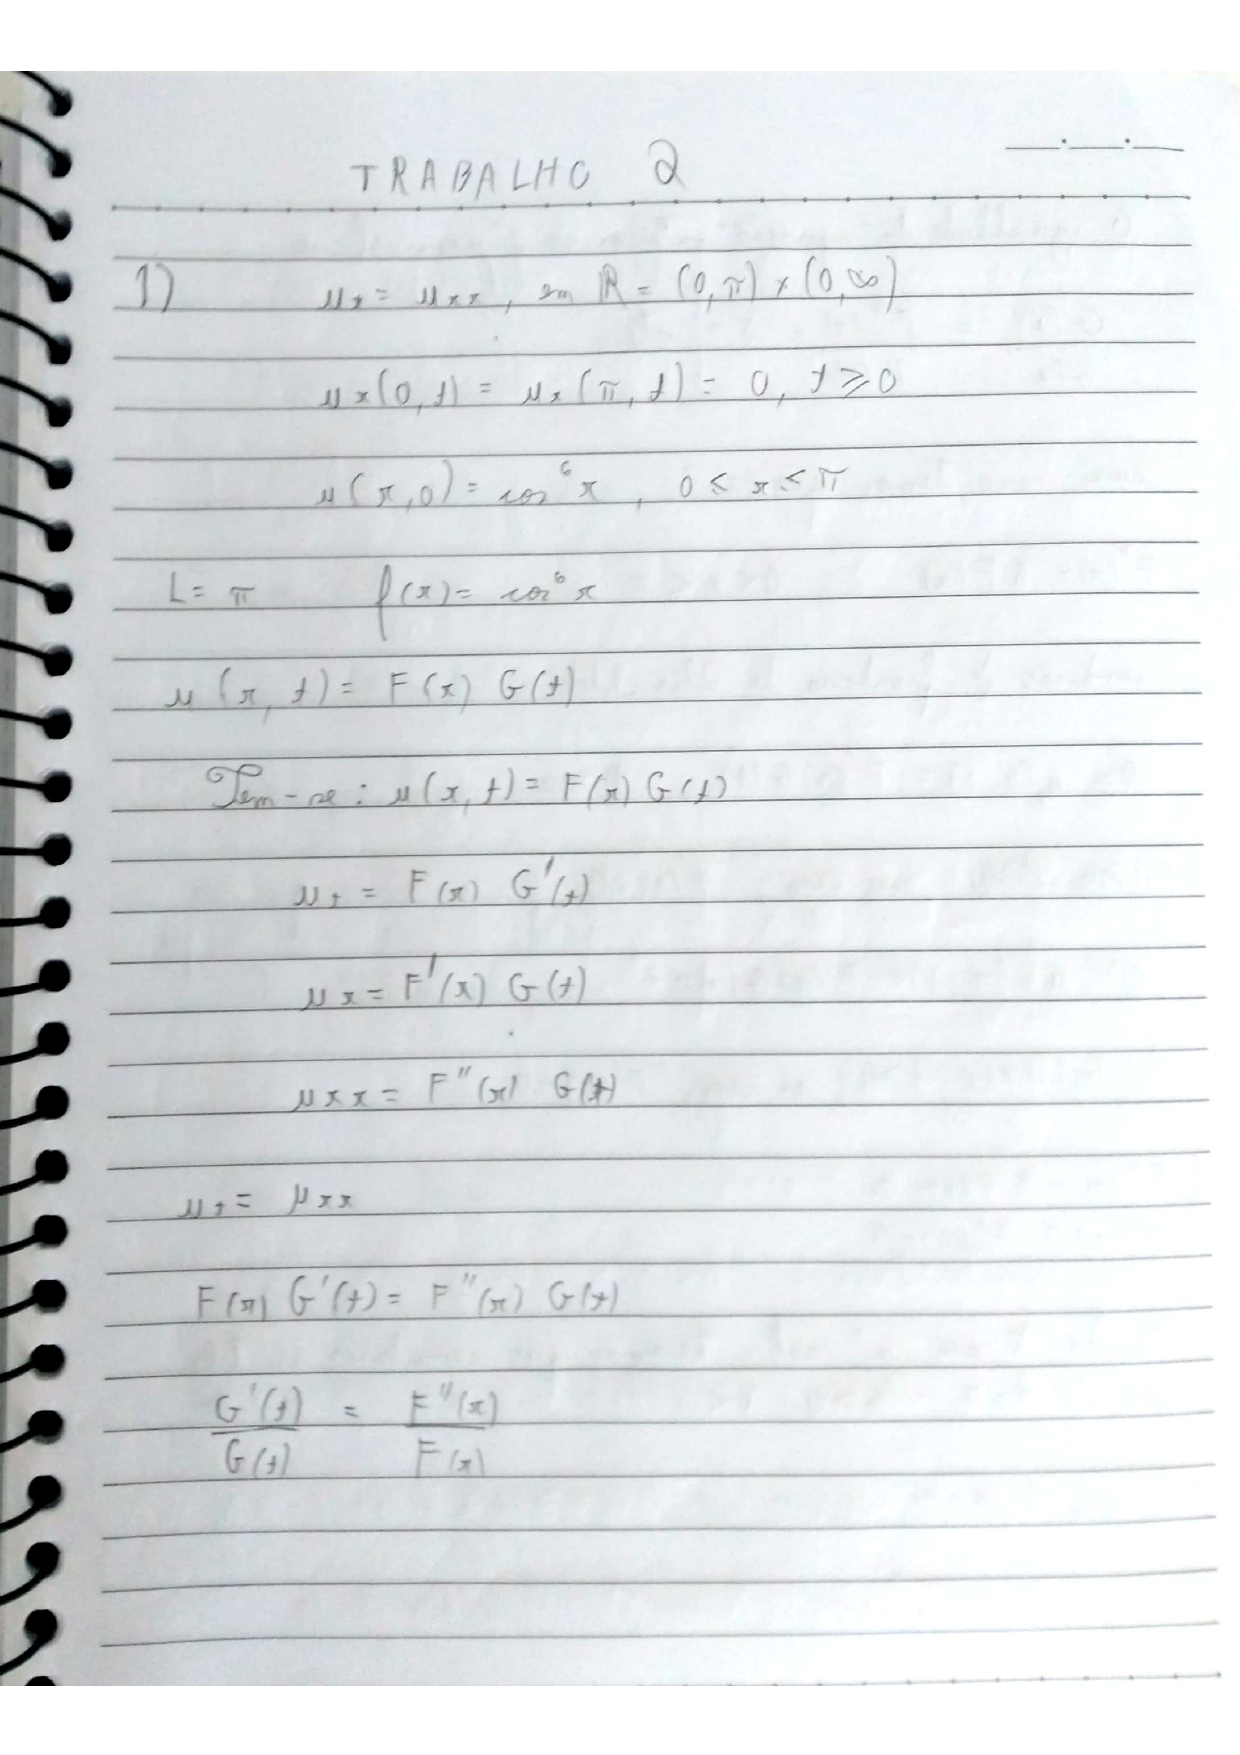
\includegraphics[width=\textwidth]{Questoes-1-3_page-0001.jpg}
        \end{wrapfigure}
                \begin{wrapfigure}{\textwidth}
            \centering
            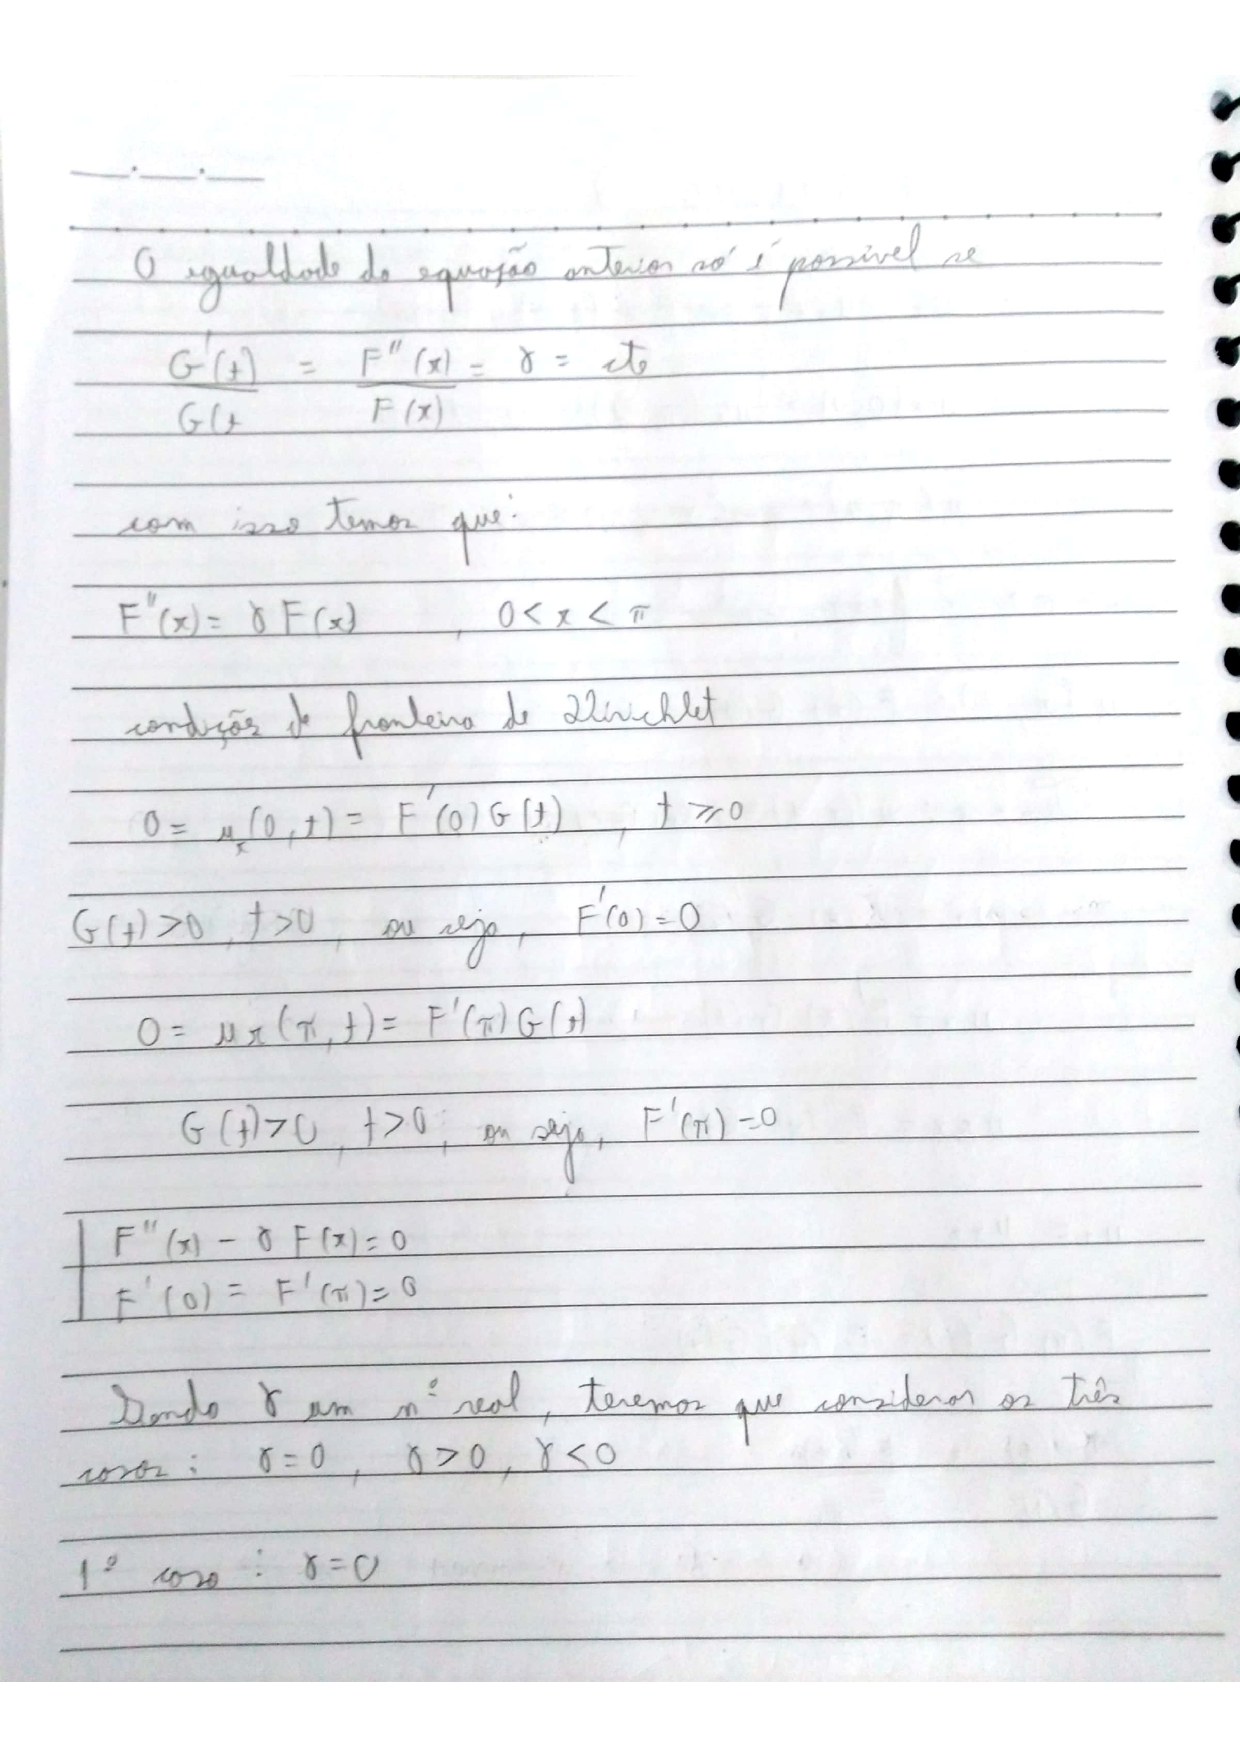
\includegraphics[width=\textwidth]{Questoes-1-3_page-0002.jpg}
        \end{wrapfigure}
        \begin{wrapfigure}{\textwidth}
            \centering
            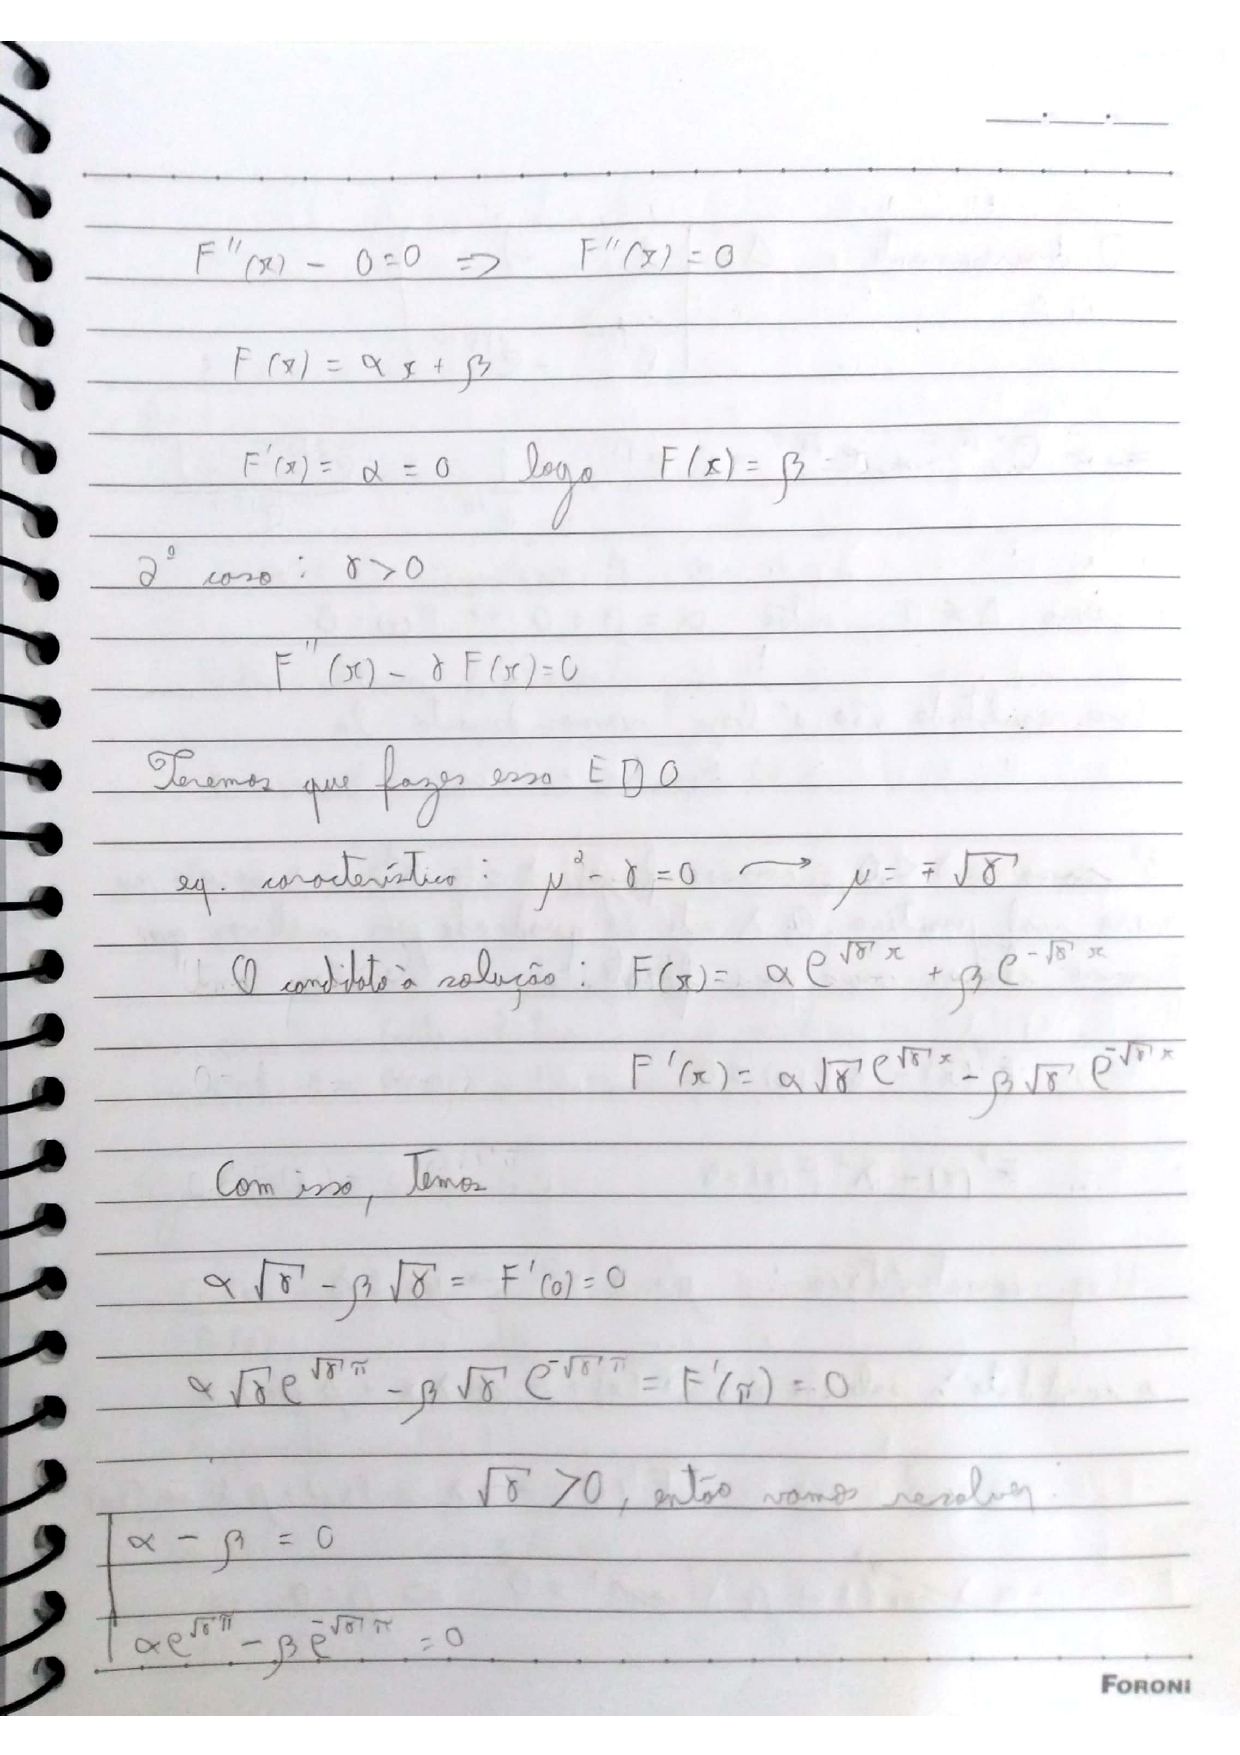
\includegraphics[width=\textwidth]{Questoes-1-3_page-0003.jpg}
        \end{wrapfigure}
        \begin{wrapfigure}{\textwidth}
            \centering
            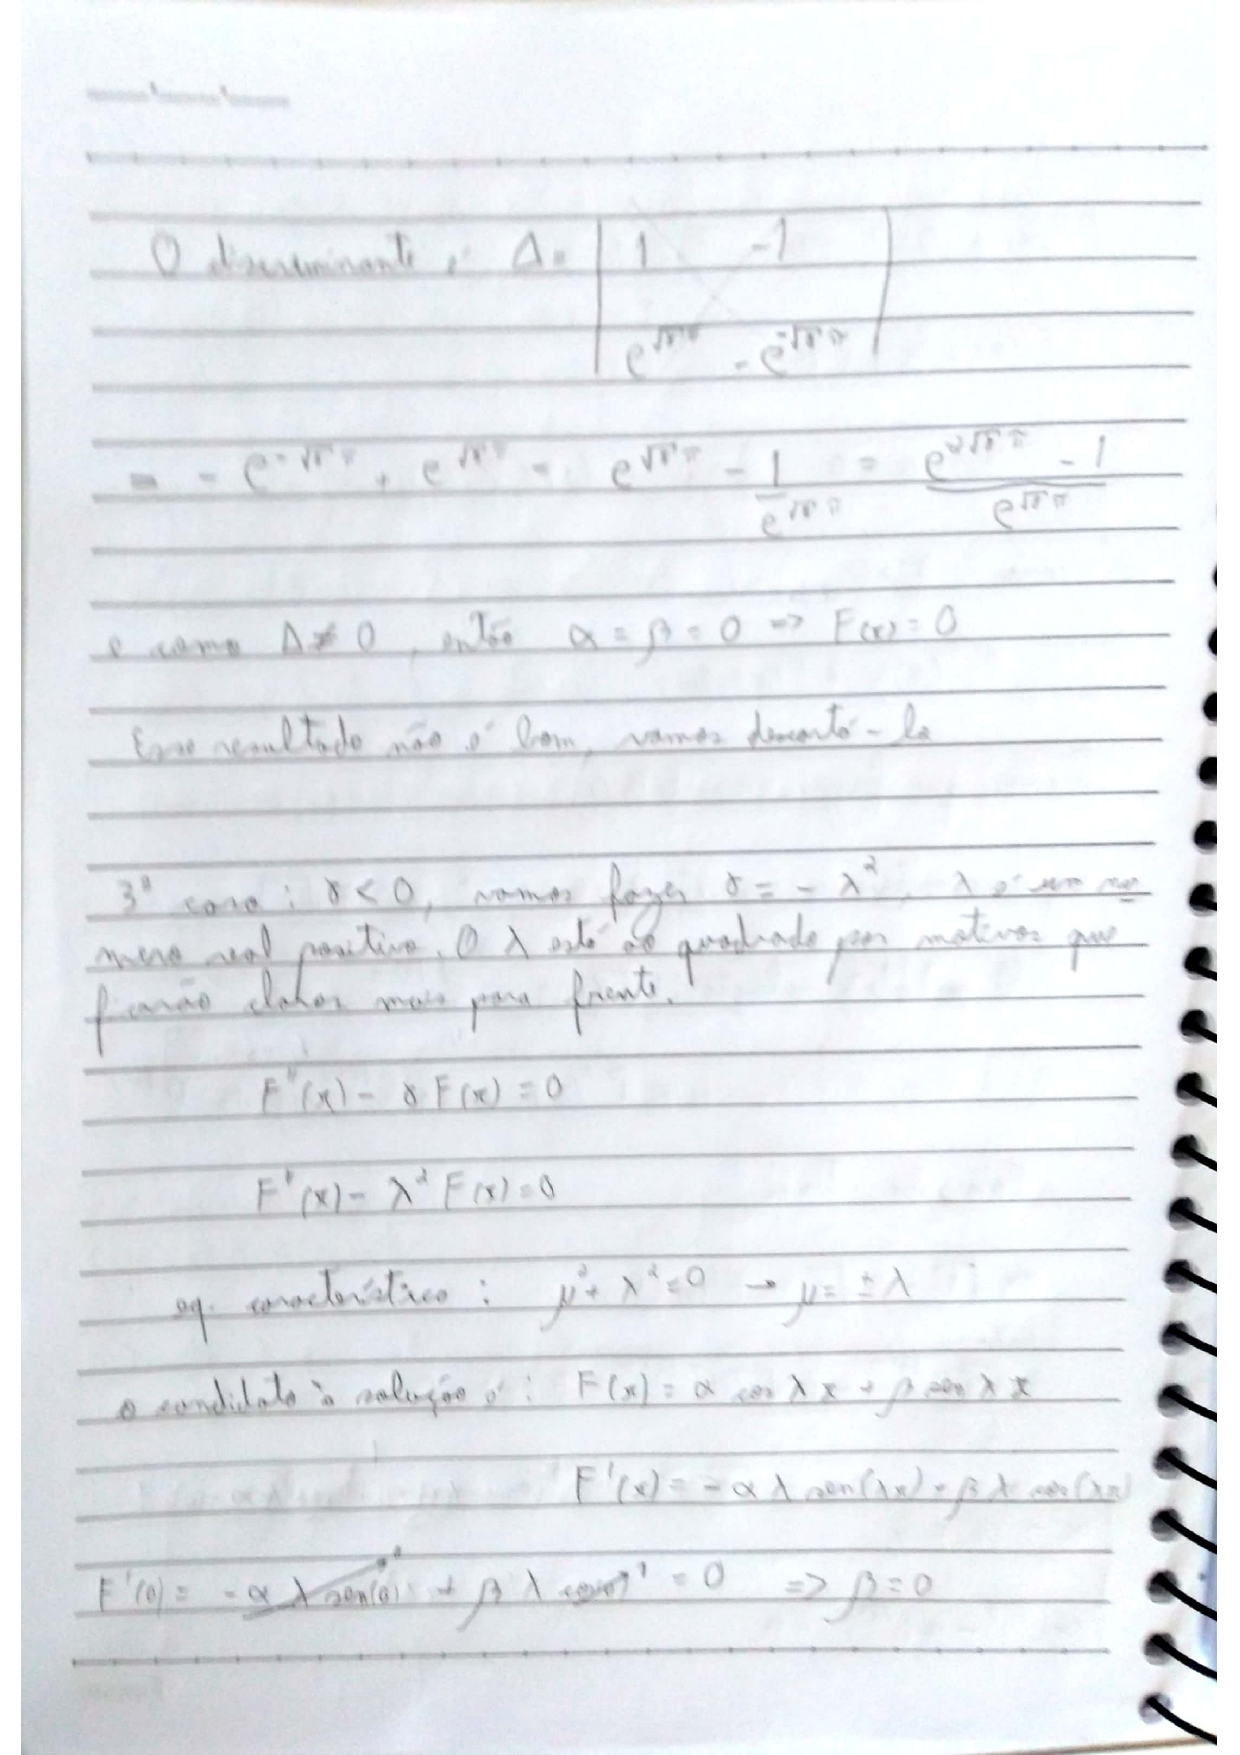
\includegraphics[width=\textwidth]{Questoes-1-3_page-0004.jpg}
        \end{wrapfigure}
                \begin{wrapfigure}{\textwidth}
            \centering
            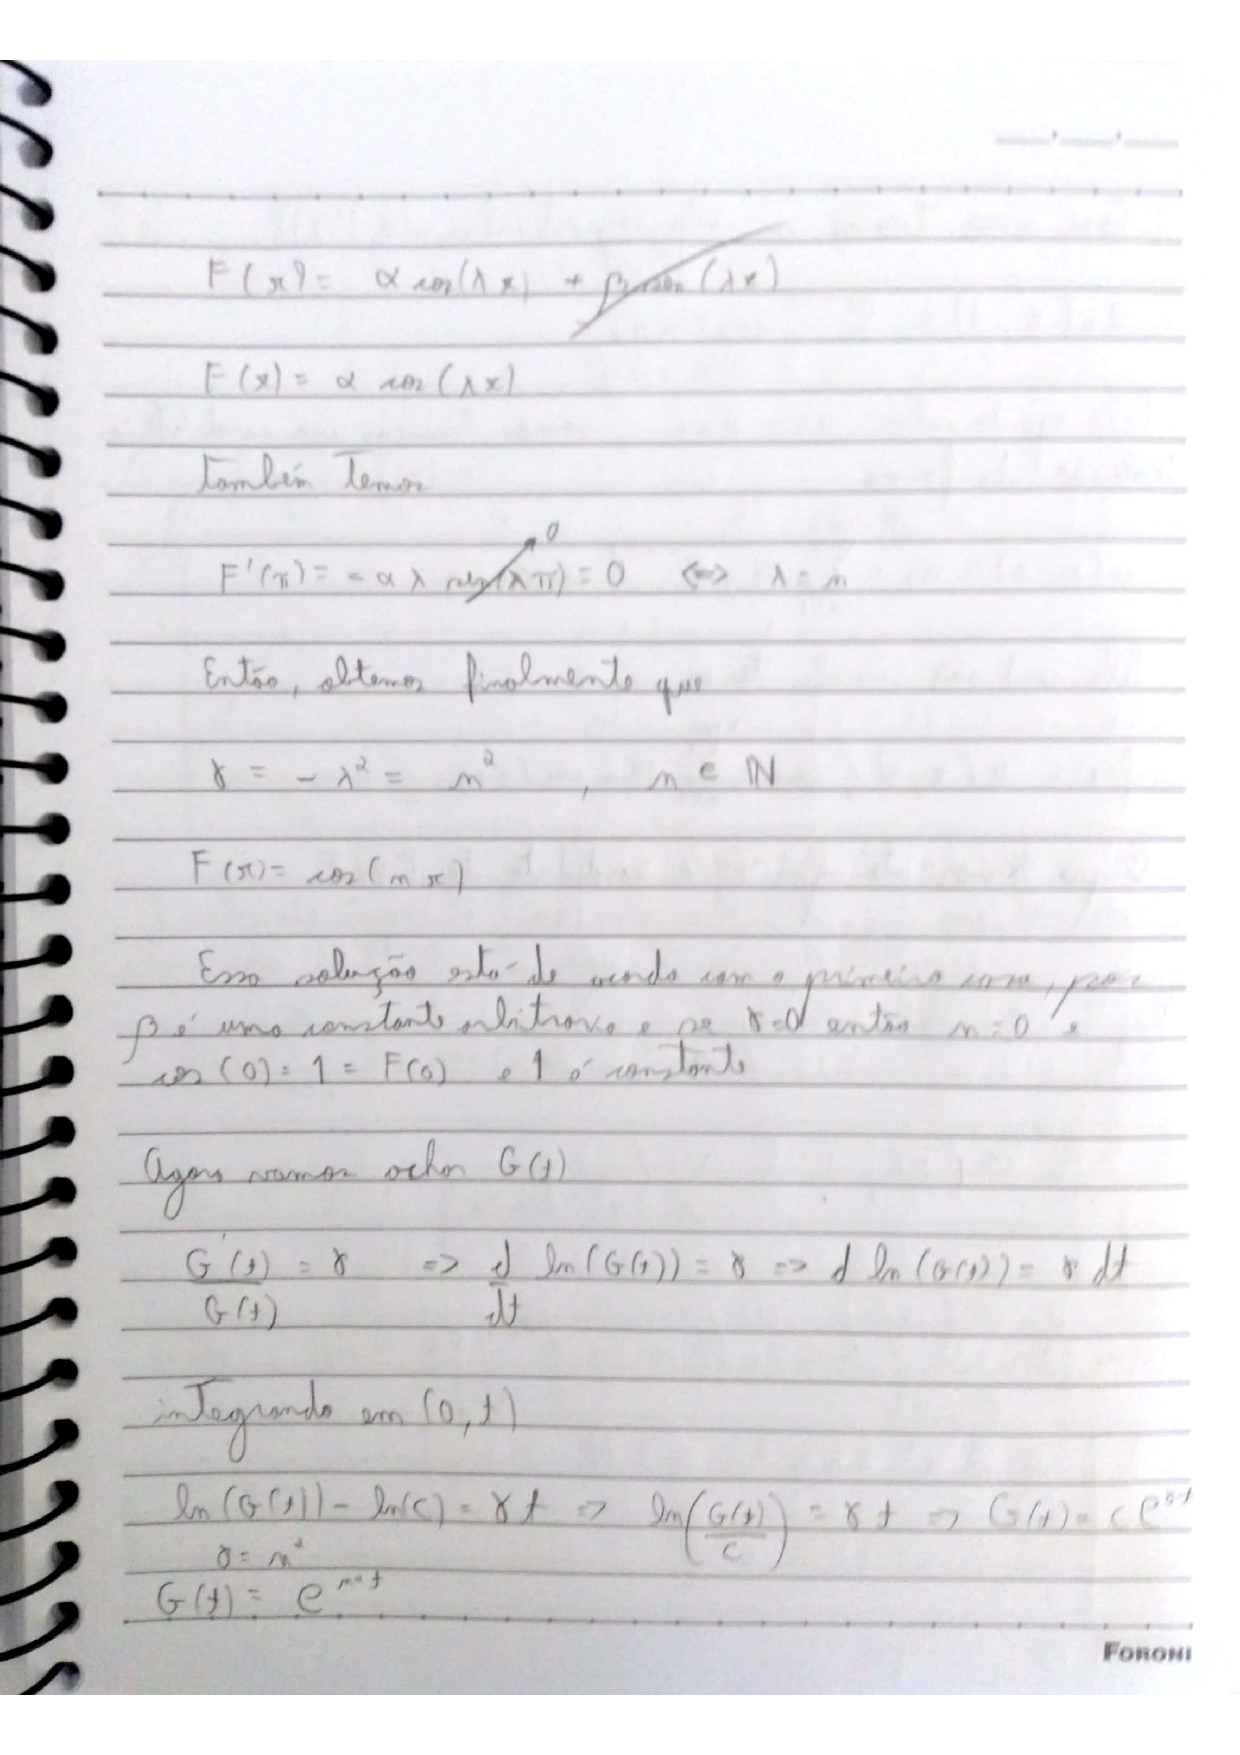
\includegraphics[width=\textwidth]{Questoes-1-3_page-0005.jpg}
        \end{wrapfigure}
                        \begin{wrapfigure}{\textwidth}
            \centering
            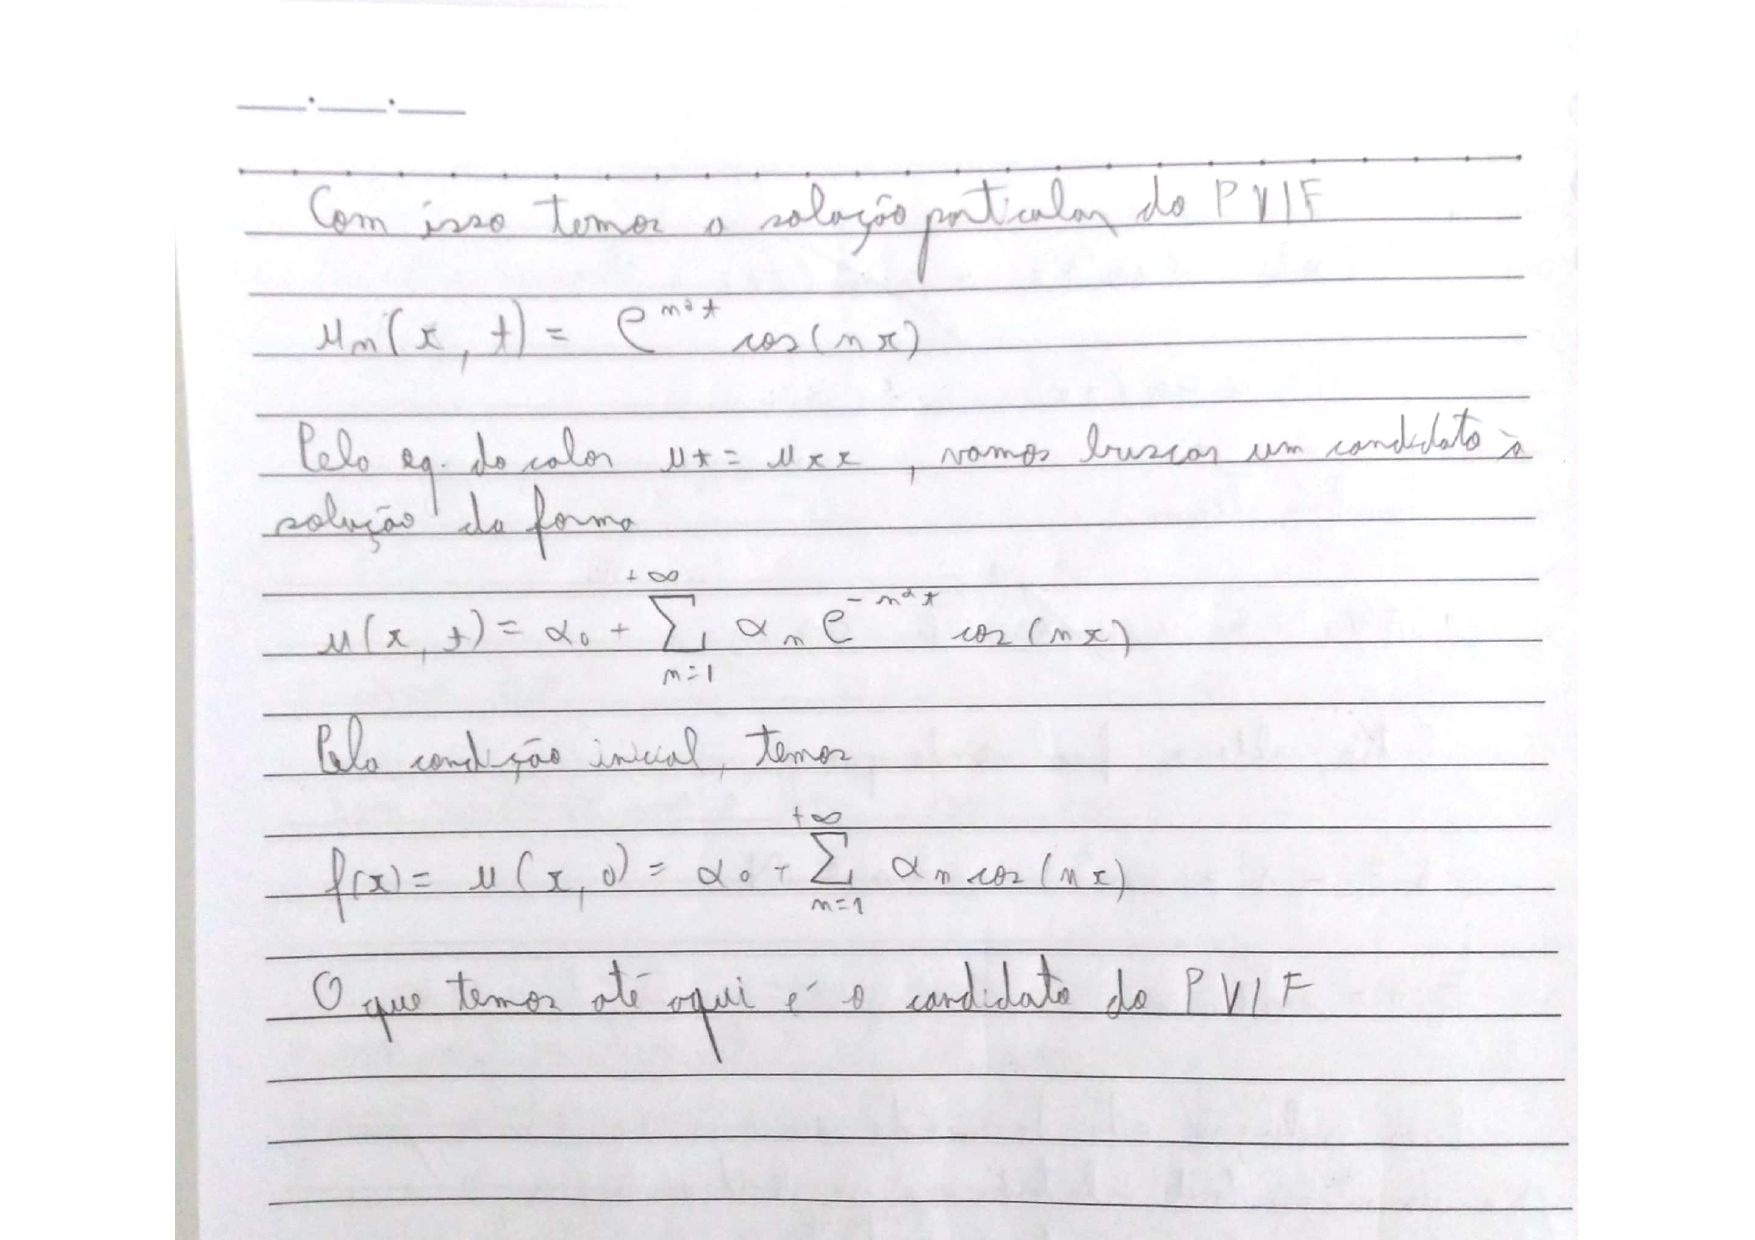
\includegraphics[width=\textwidth]{Questoes-1-3_page-0006.jpg}
        \end{wrapfigure}




    \section{}

        \begin{wrapfigure}{\textwidth}
            \centering
            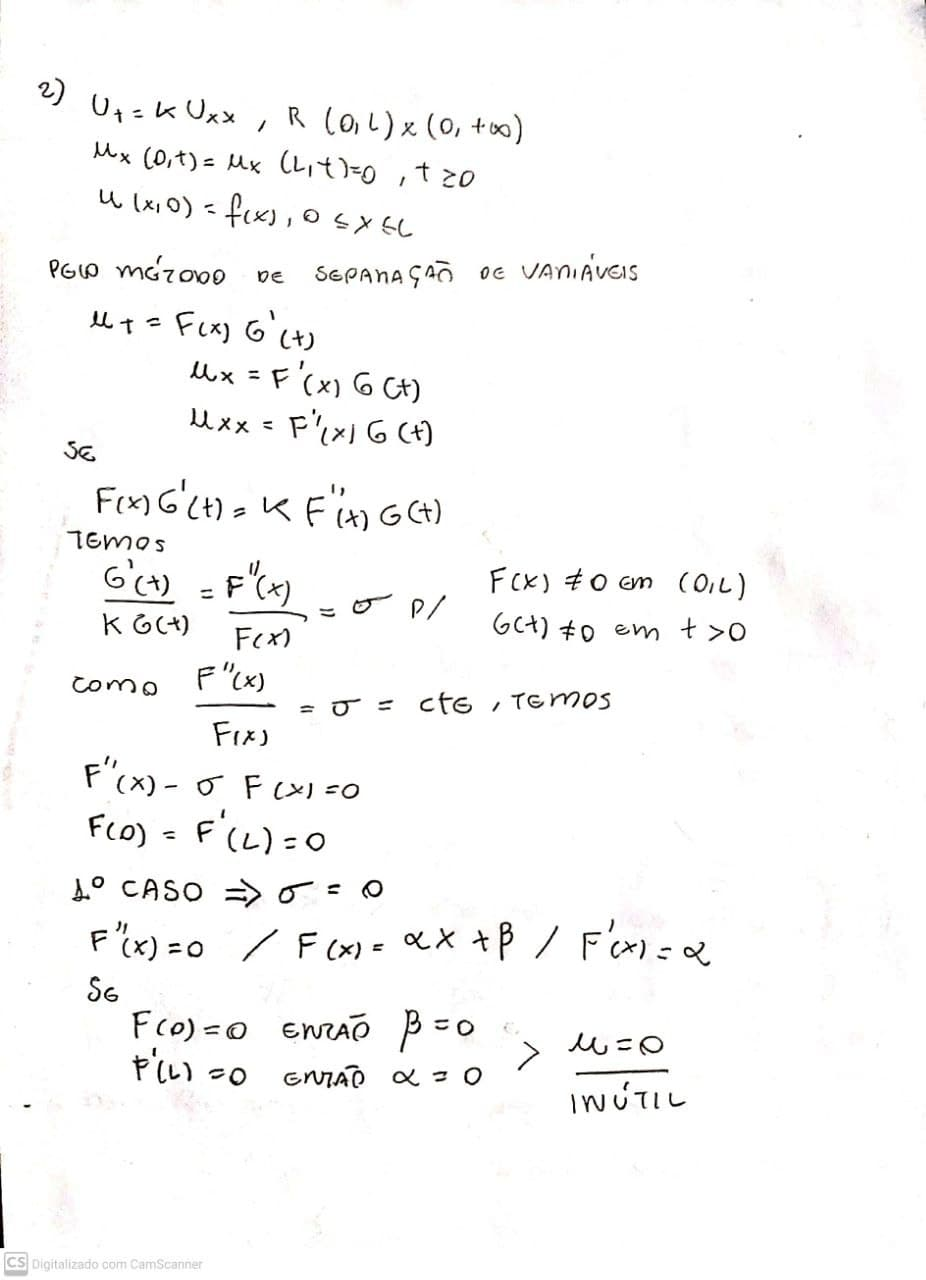
\includegraphics[width=\textwidth]{21.jpg}
        \end{wrapfigure}
        \begin{wrapfigure}{\textwidth}
            \centering
            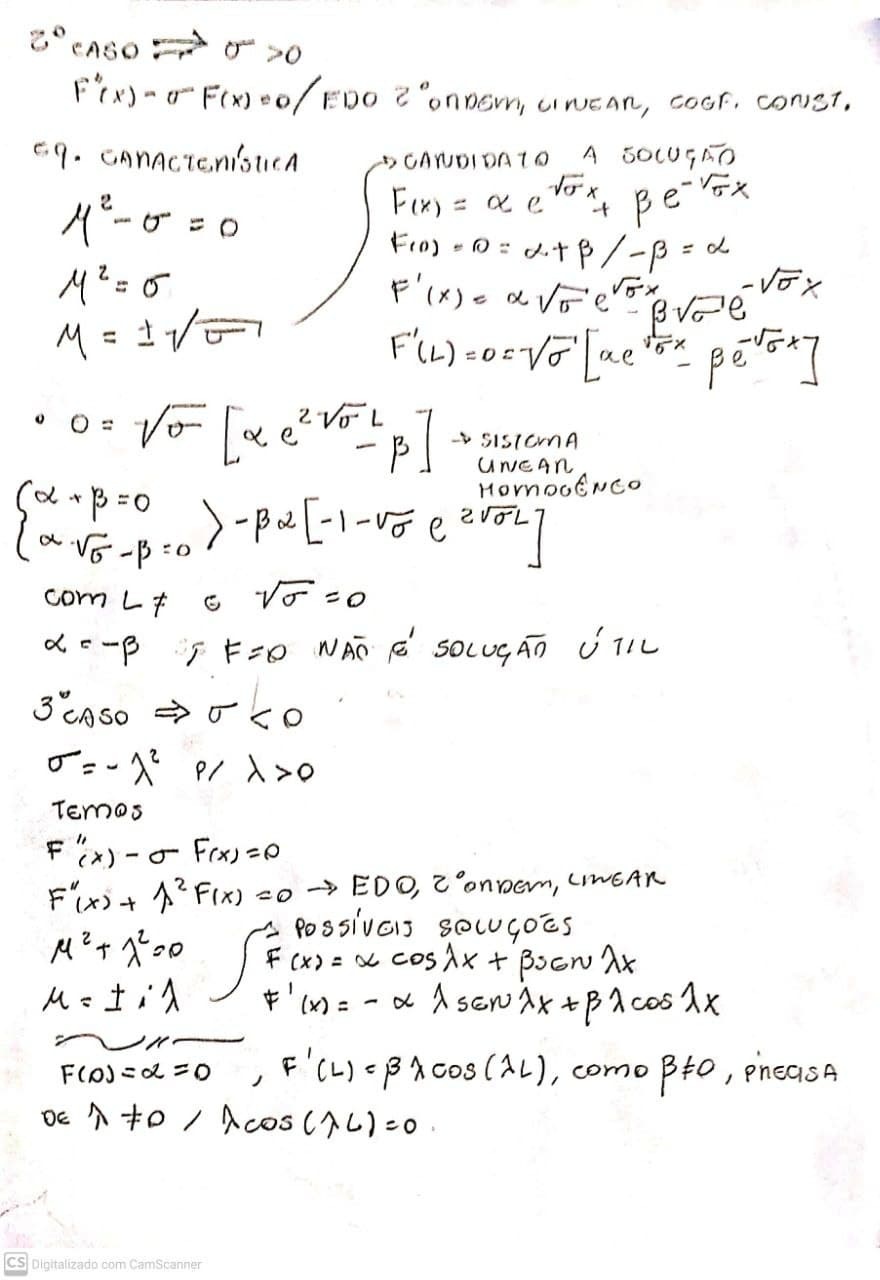
\includegraphics[width=\textwidth]{22.jpg}
        \end{wrapfigure}
        \begin{wrapfigure}{\textwidth}
            \centering
            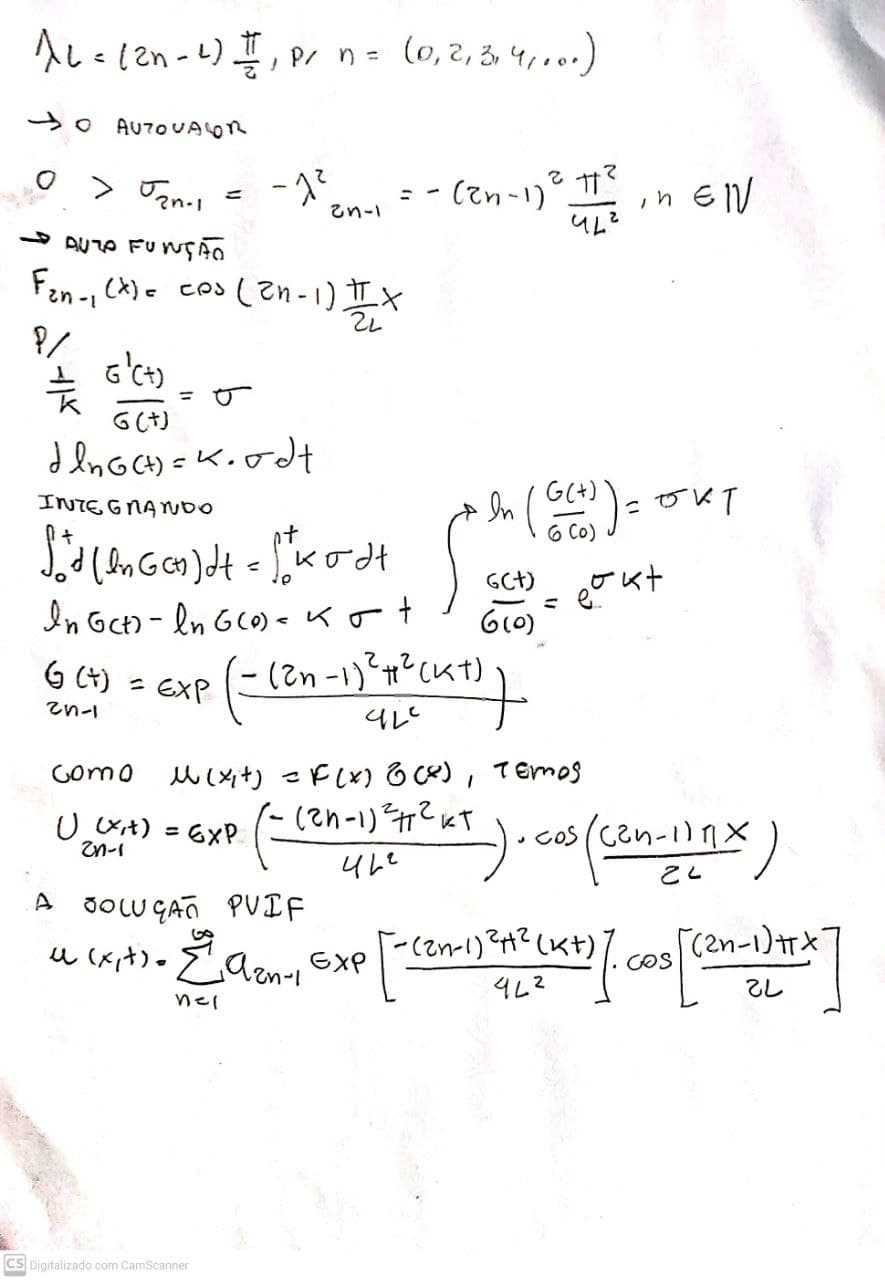
\includegraphics[width=\textwidth]{23.jpg}
        \end{wrapfigure}

    
    \section{} 
        \begin{wrapfigure}{\textwidth}
            \centering
            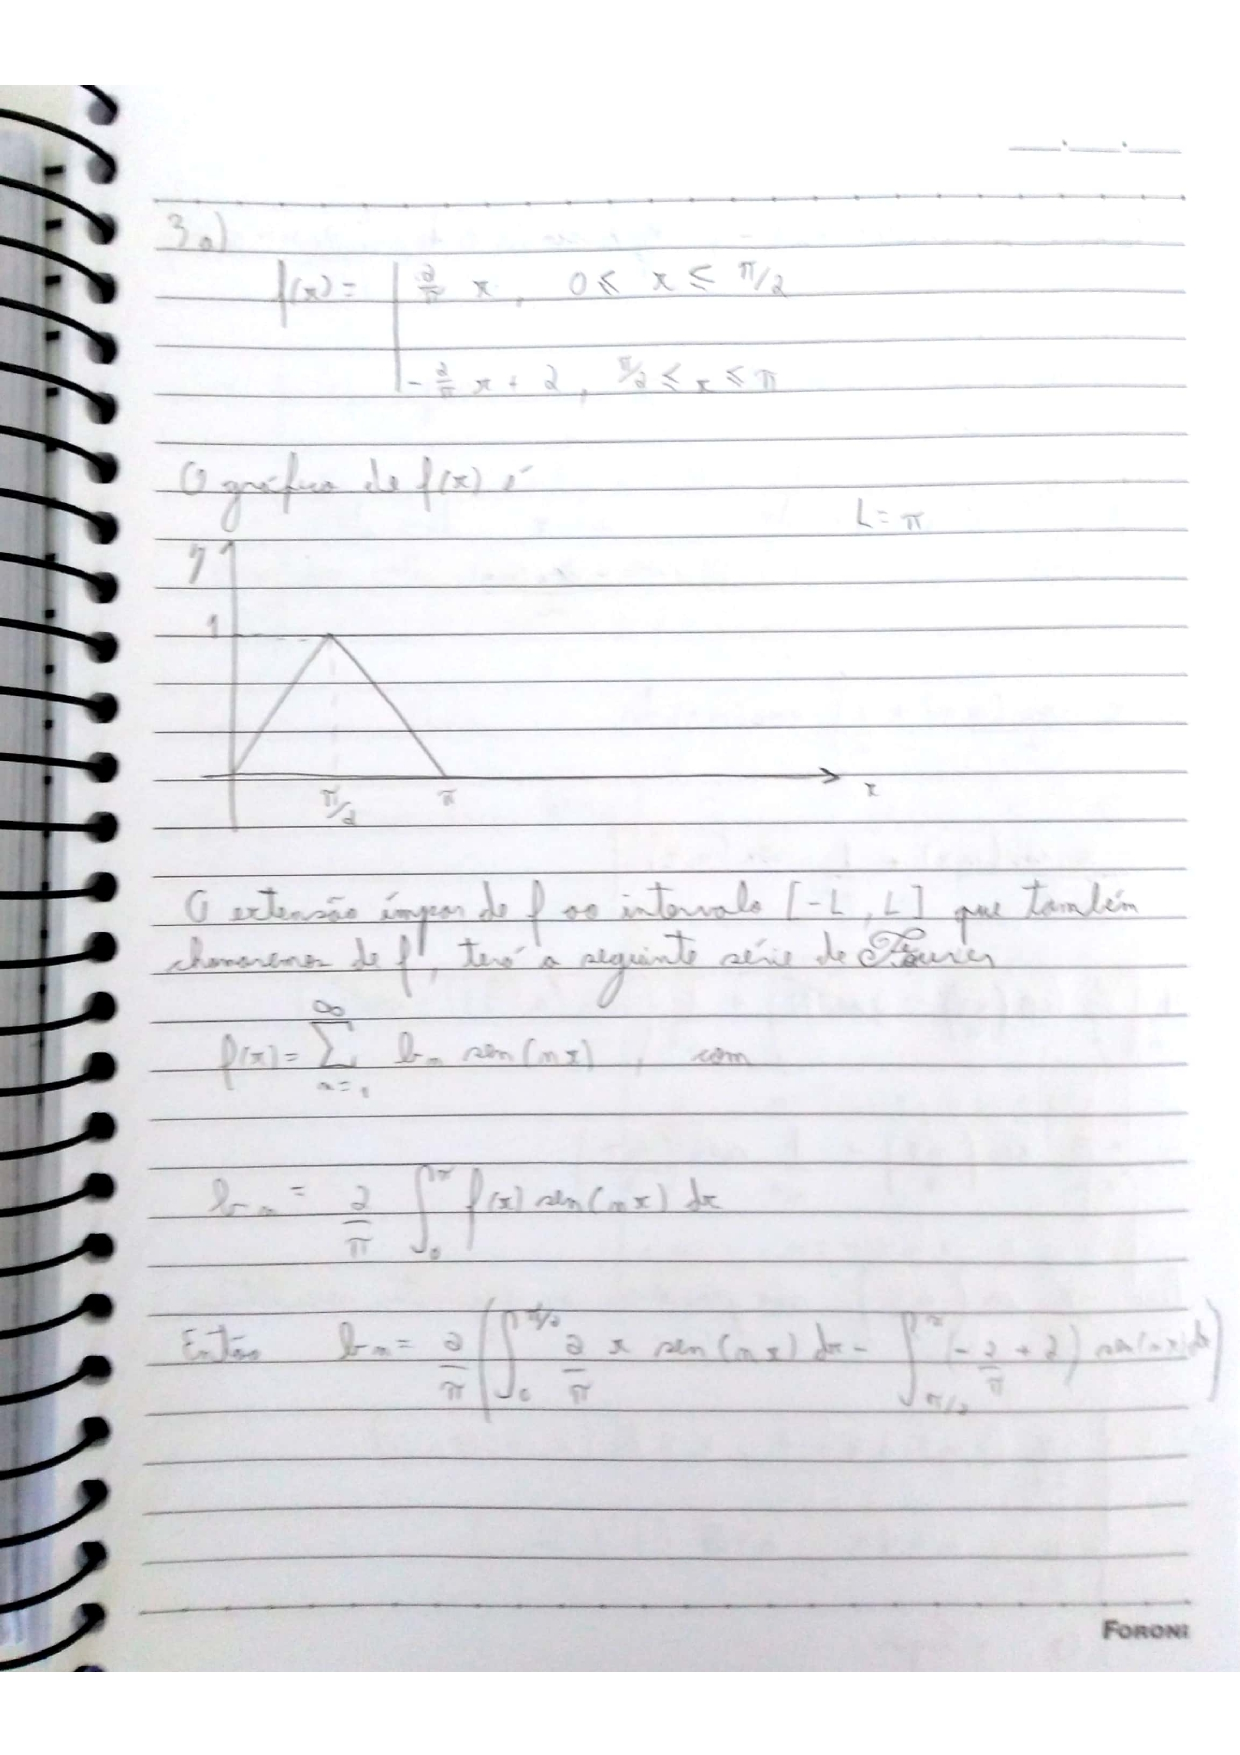
\includegraphics[width=\textwidth]{Questoes-1-3_page-0007.jpg}
        \end{wrapfigure}
        \begin{wrapfigure}{\textwidth}
            \centering
            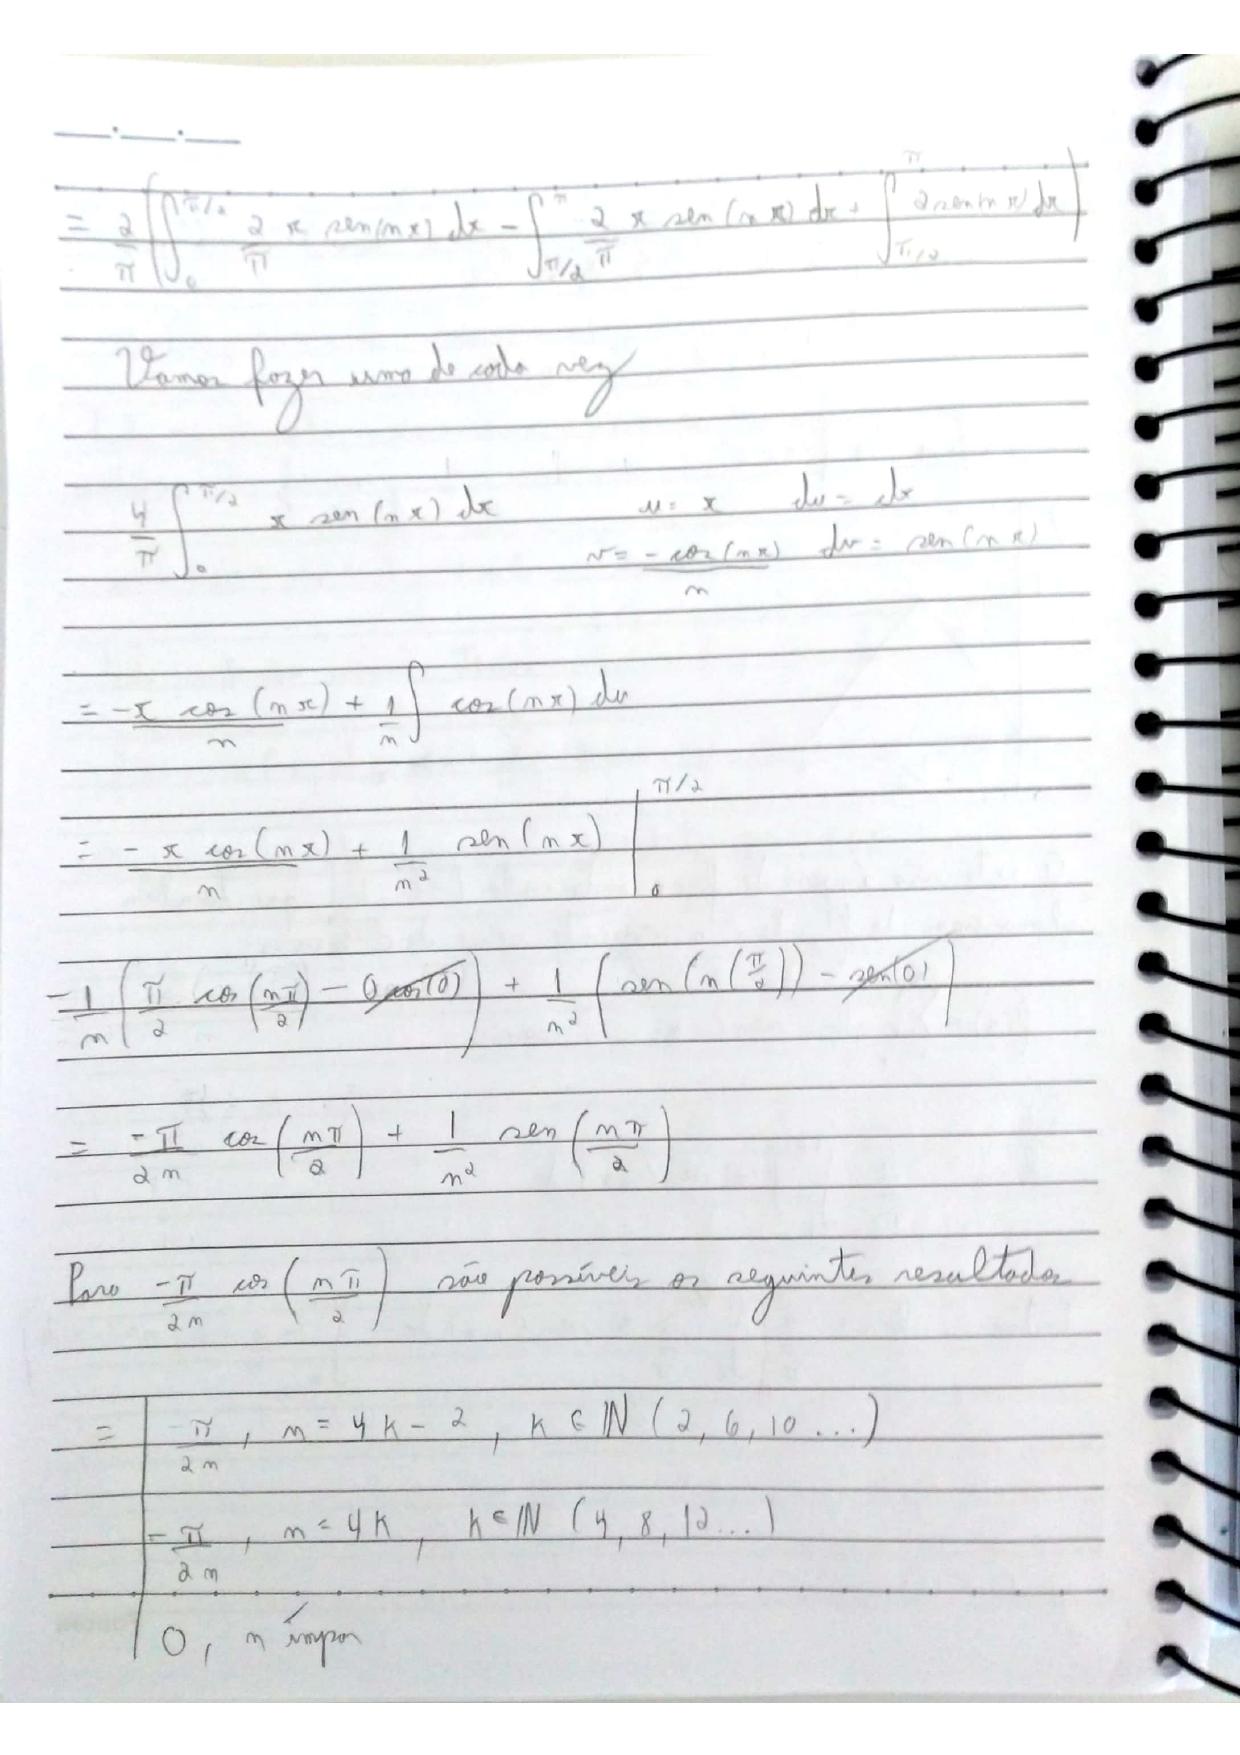
\includegraphics[width=\textwidth]{Questoes-1-3_page-0008.jpg}
        \end{wrapfigure}
        \begin{wrapfigure}{\textwidth}
            \centering
            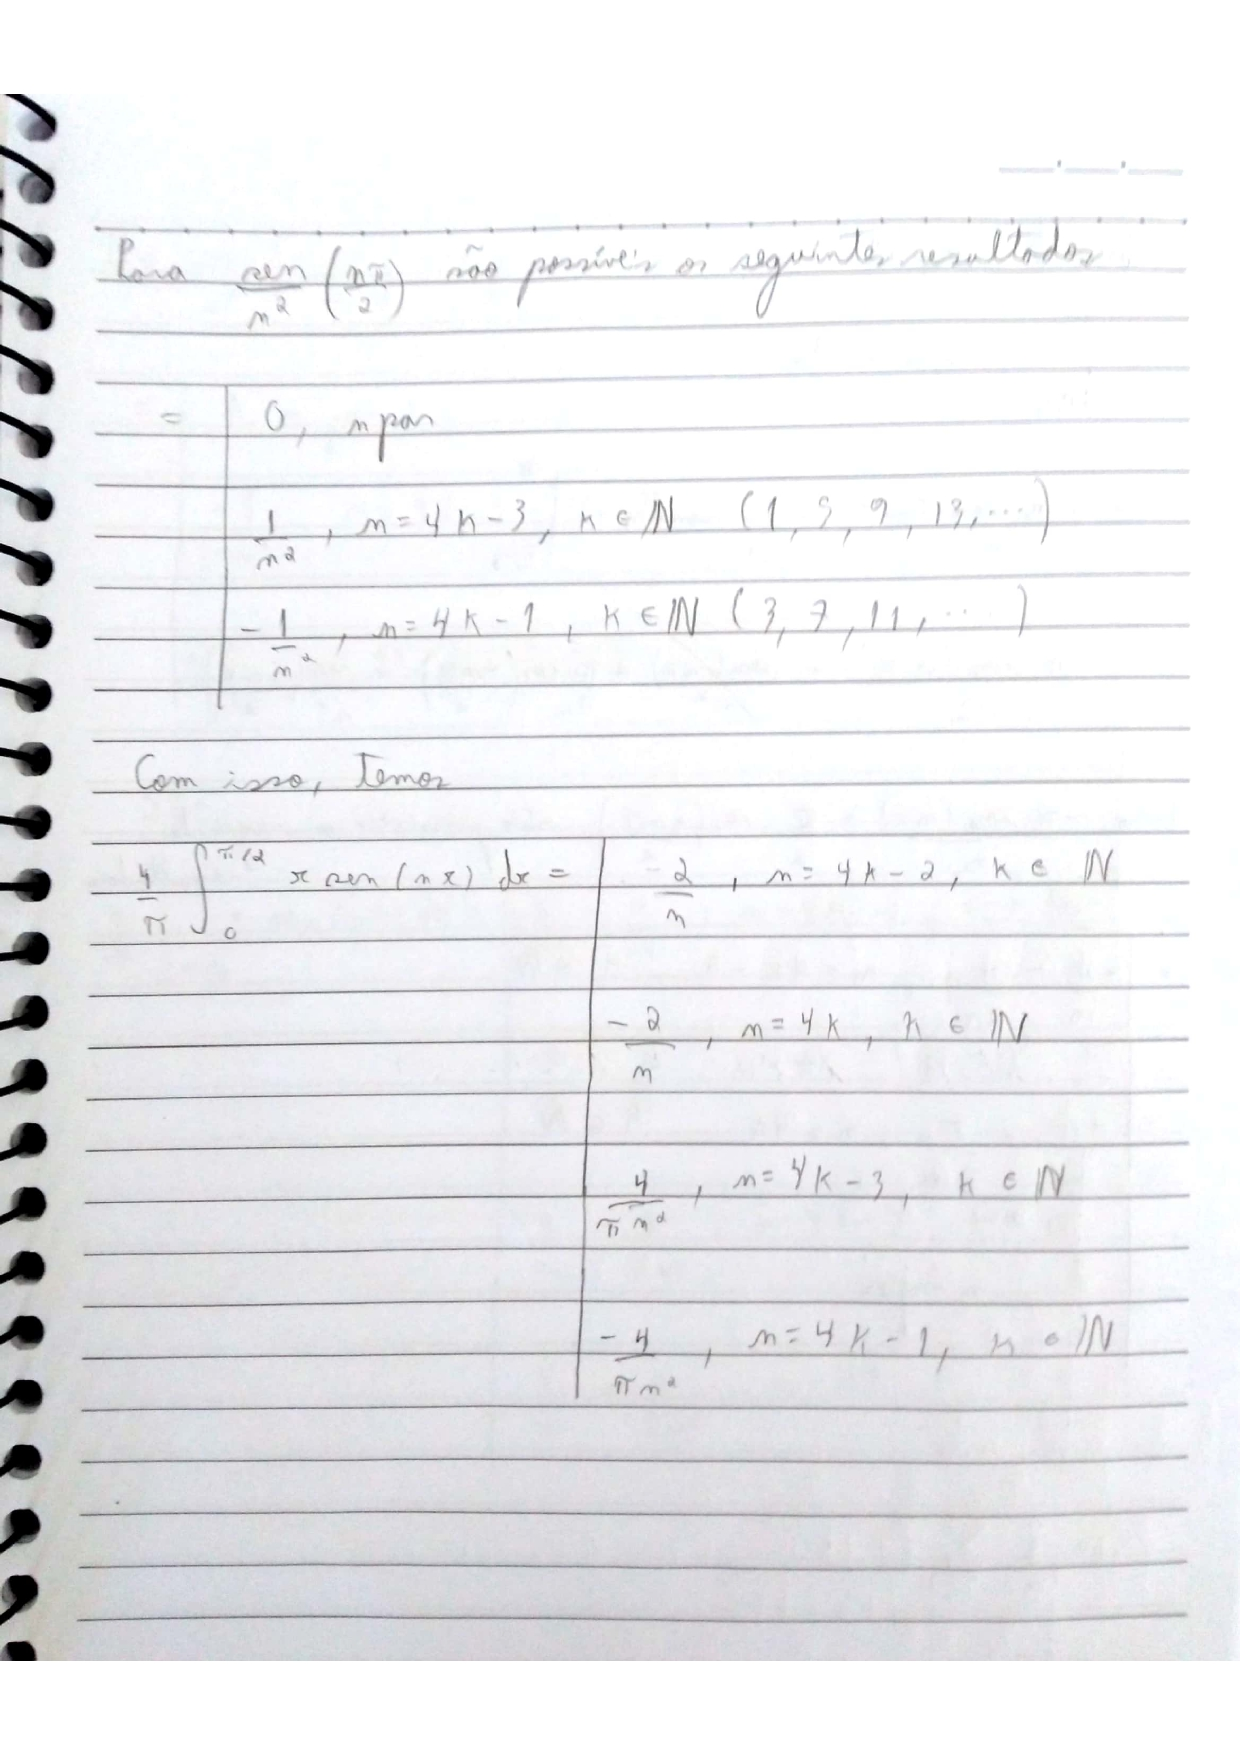
\includegraphics[width=\textwidth]{Questoes-1-3_page-0009.jpg}
        \end{wrapfigure}
        \begin{wrapfigure}{\textwidth}
            \centering
            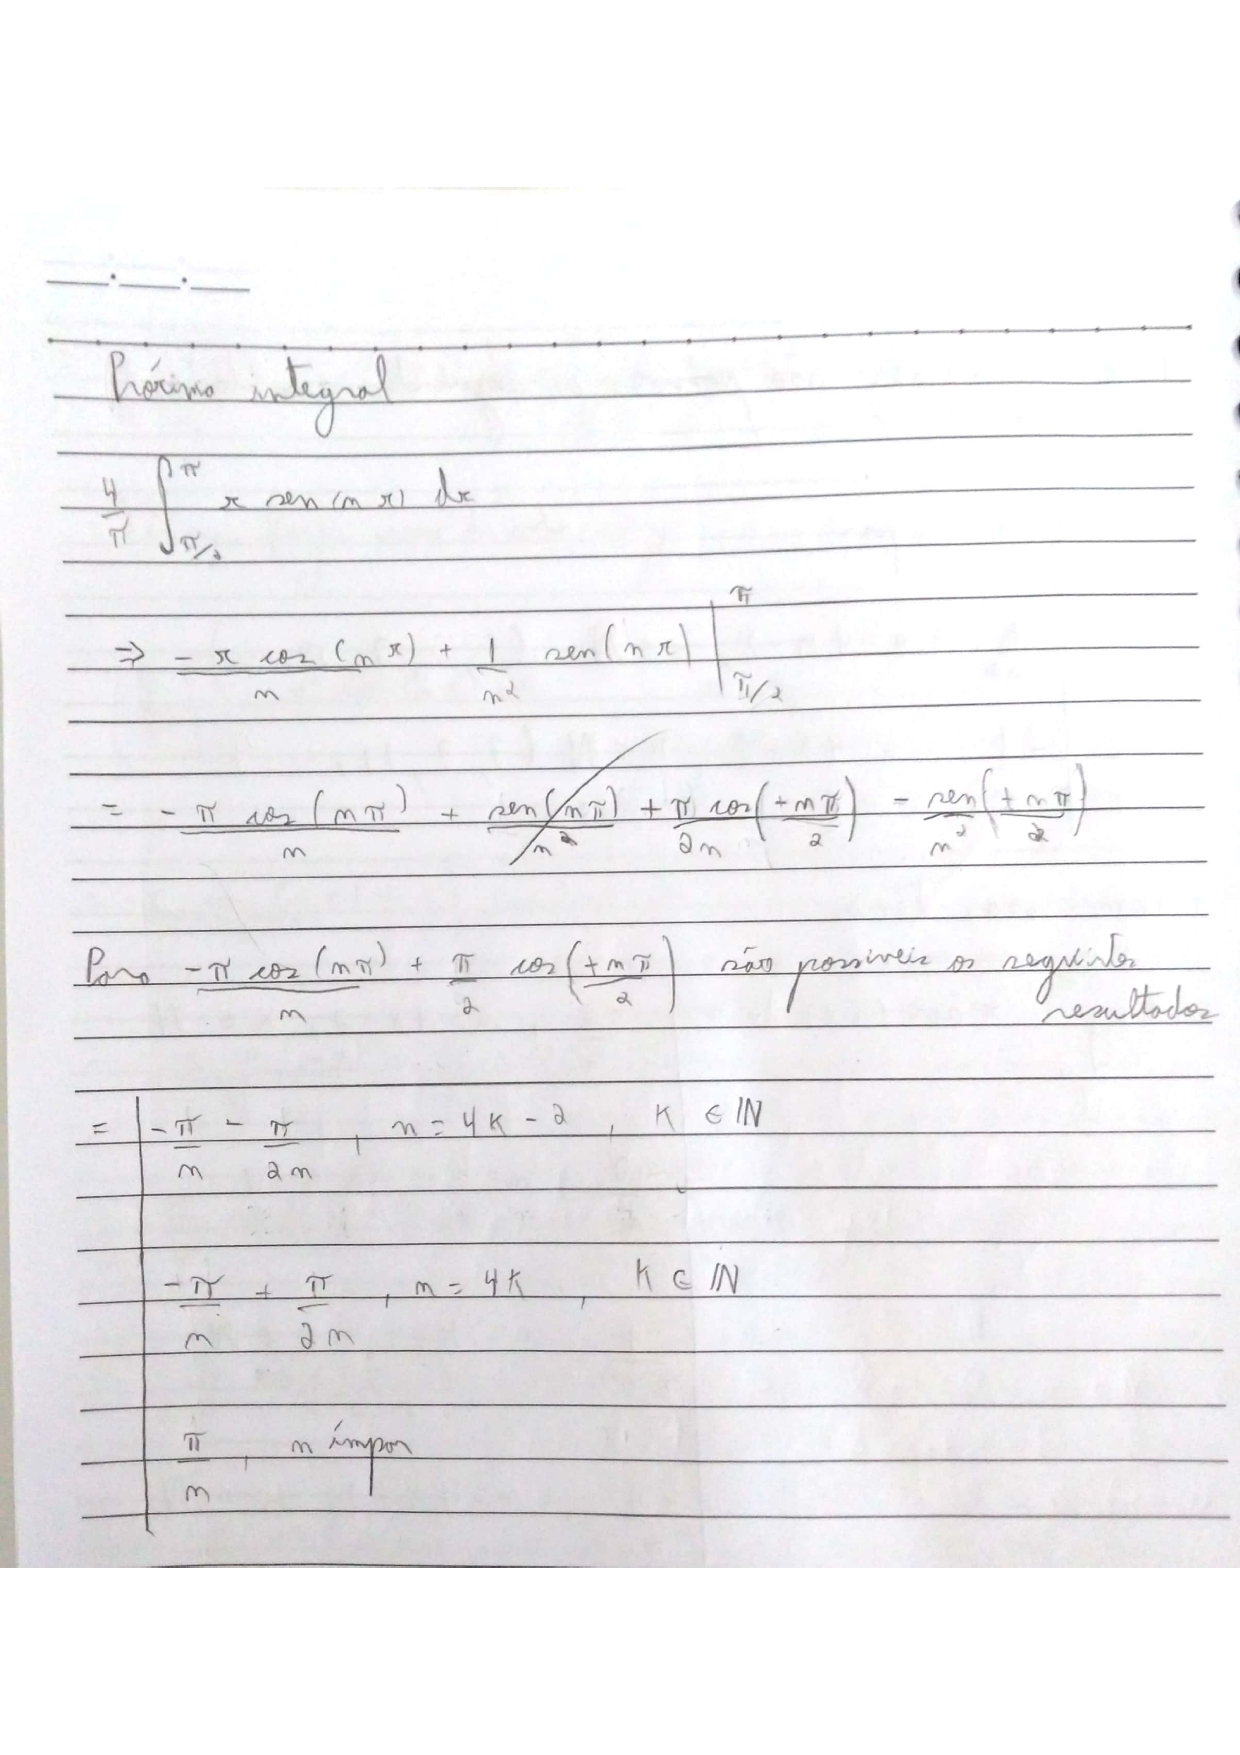
\includegraphics[width=\textwidth]{Questoes-1-3_page-0010.jpg}
        \end{wrapfigure}
                \begin{wrapfigure}{\textwidth}
            \centering
            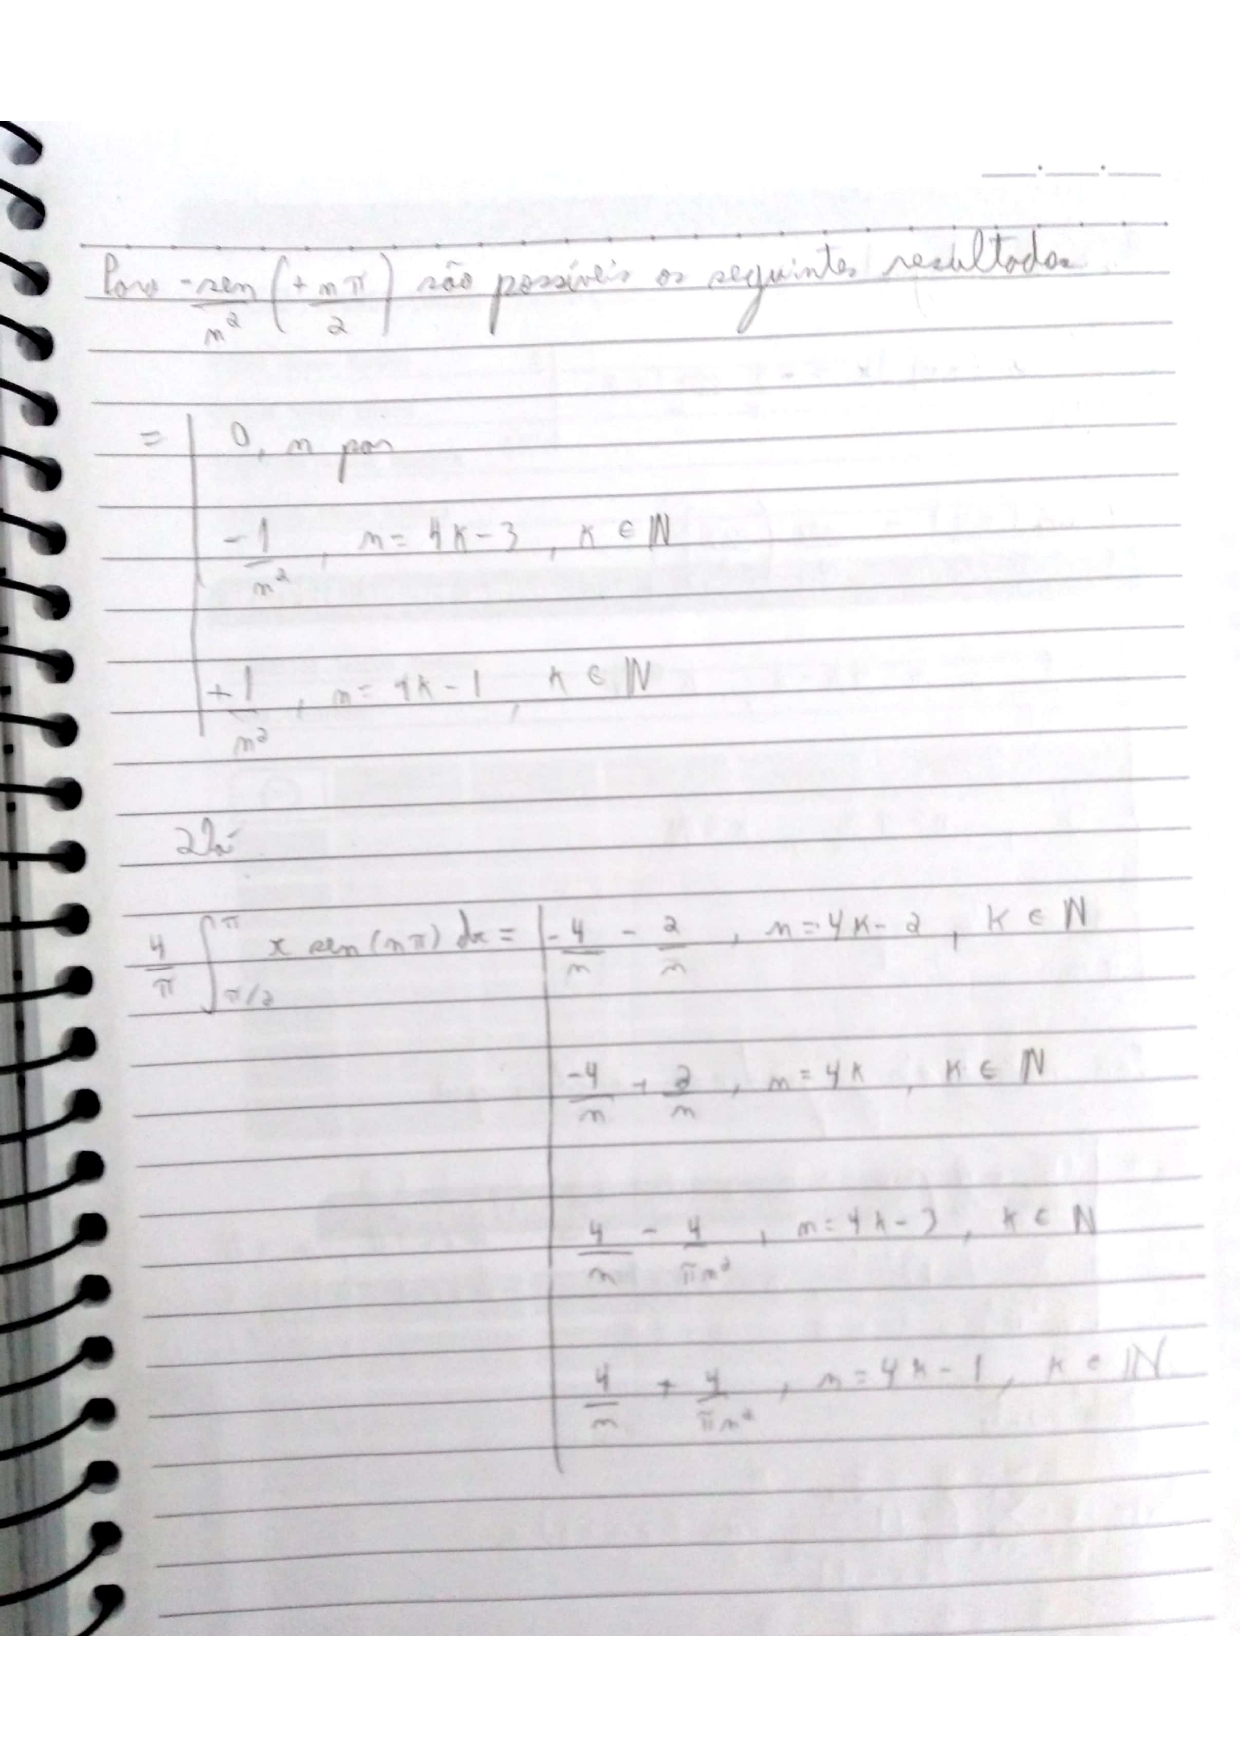
\includegraphics[width=\textwidth]{Questoes-1-3_page-0011.jpg}
        \end{wrapfigure}
        \begin{wrapfigure}{\textwidth}
            \centering
            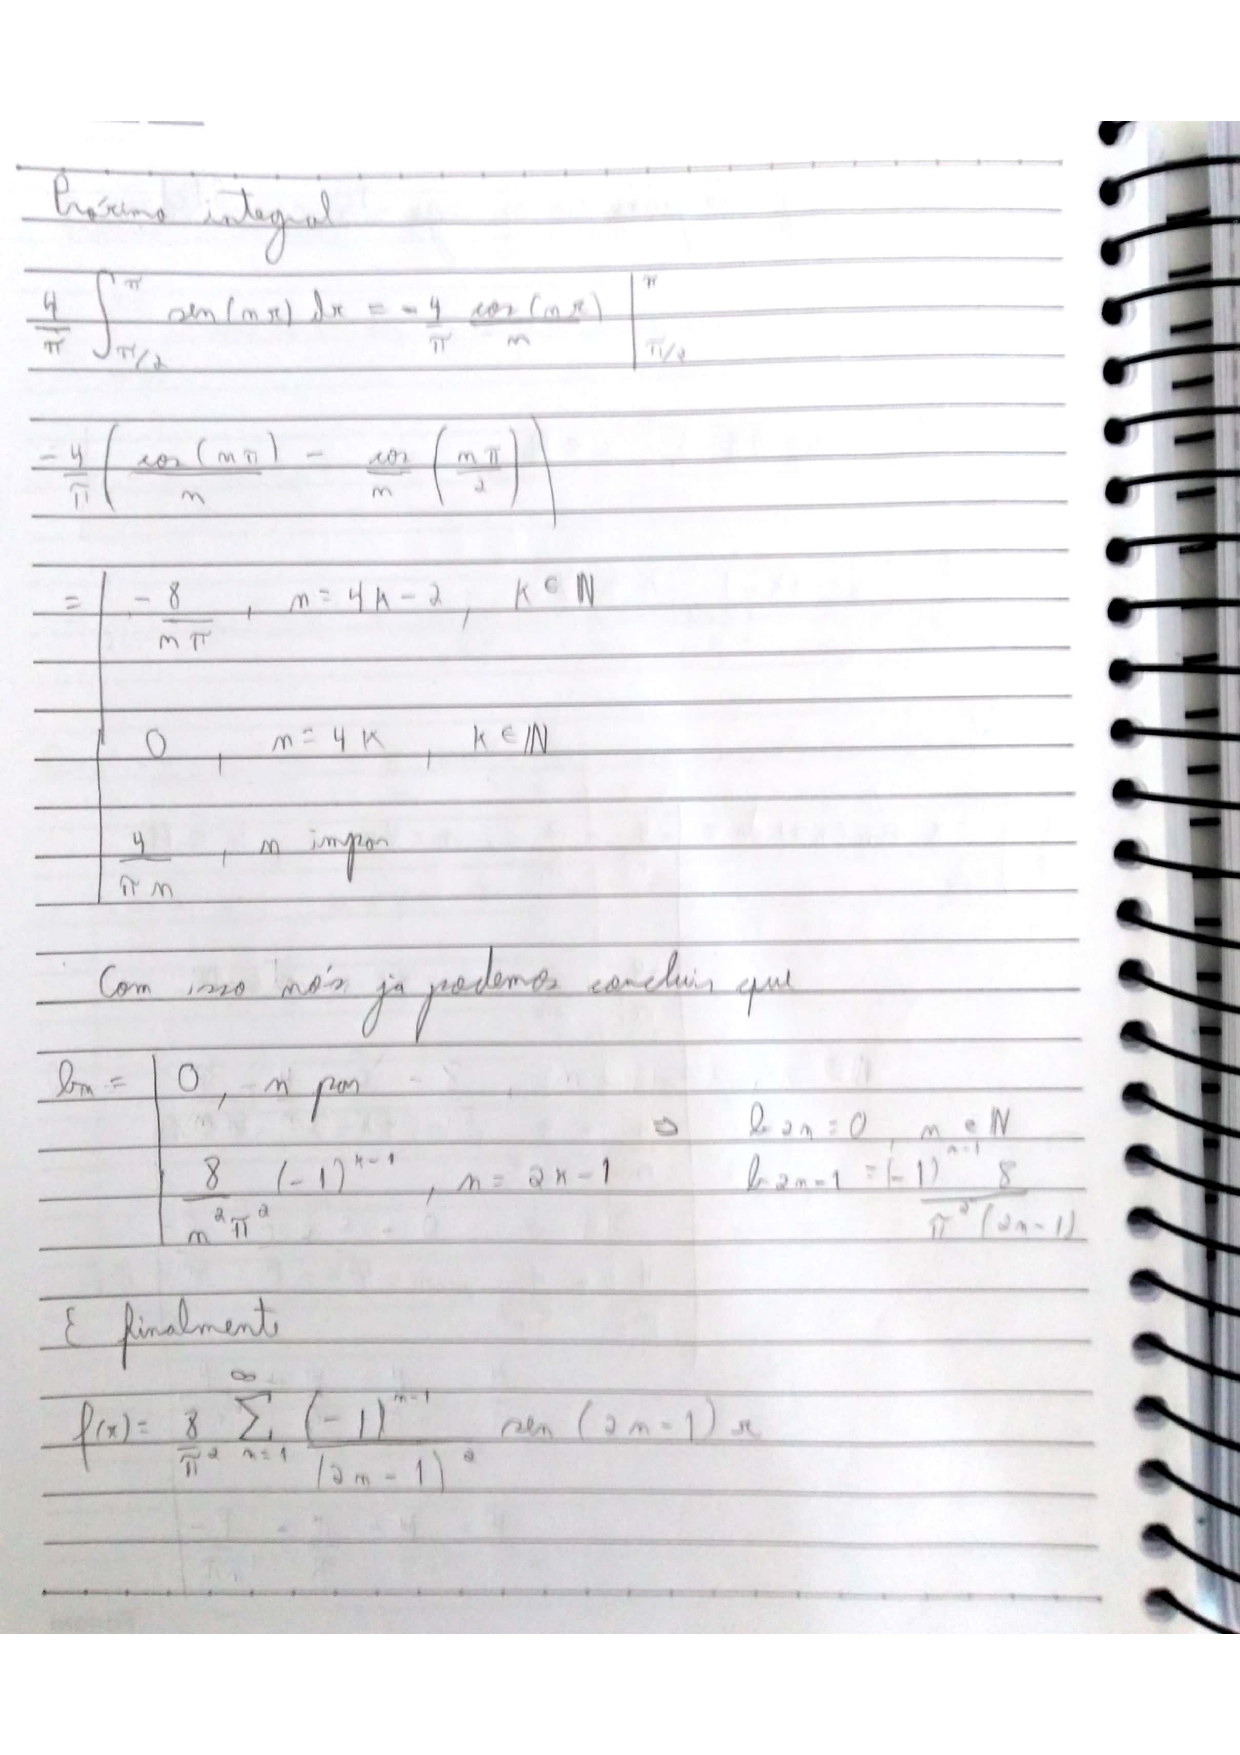
\includegraphics[width=\textwidth]{Questoes-1-3_page-0012.jpg}
        \end{wrapfigure}
        \begin{wrapfigure}{\textwidth}
            \centering
            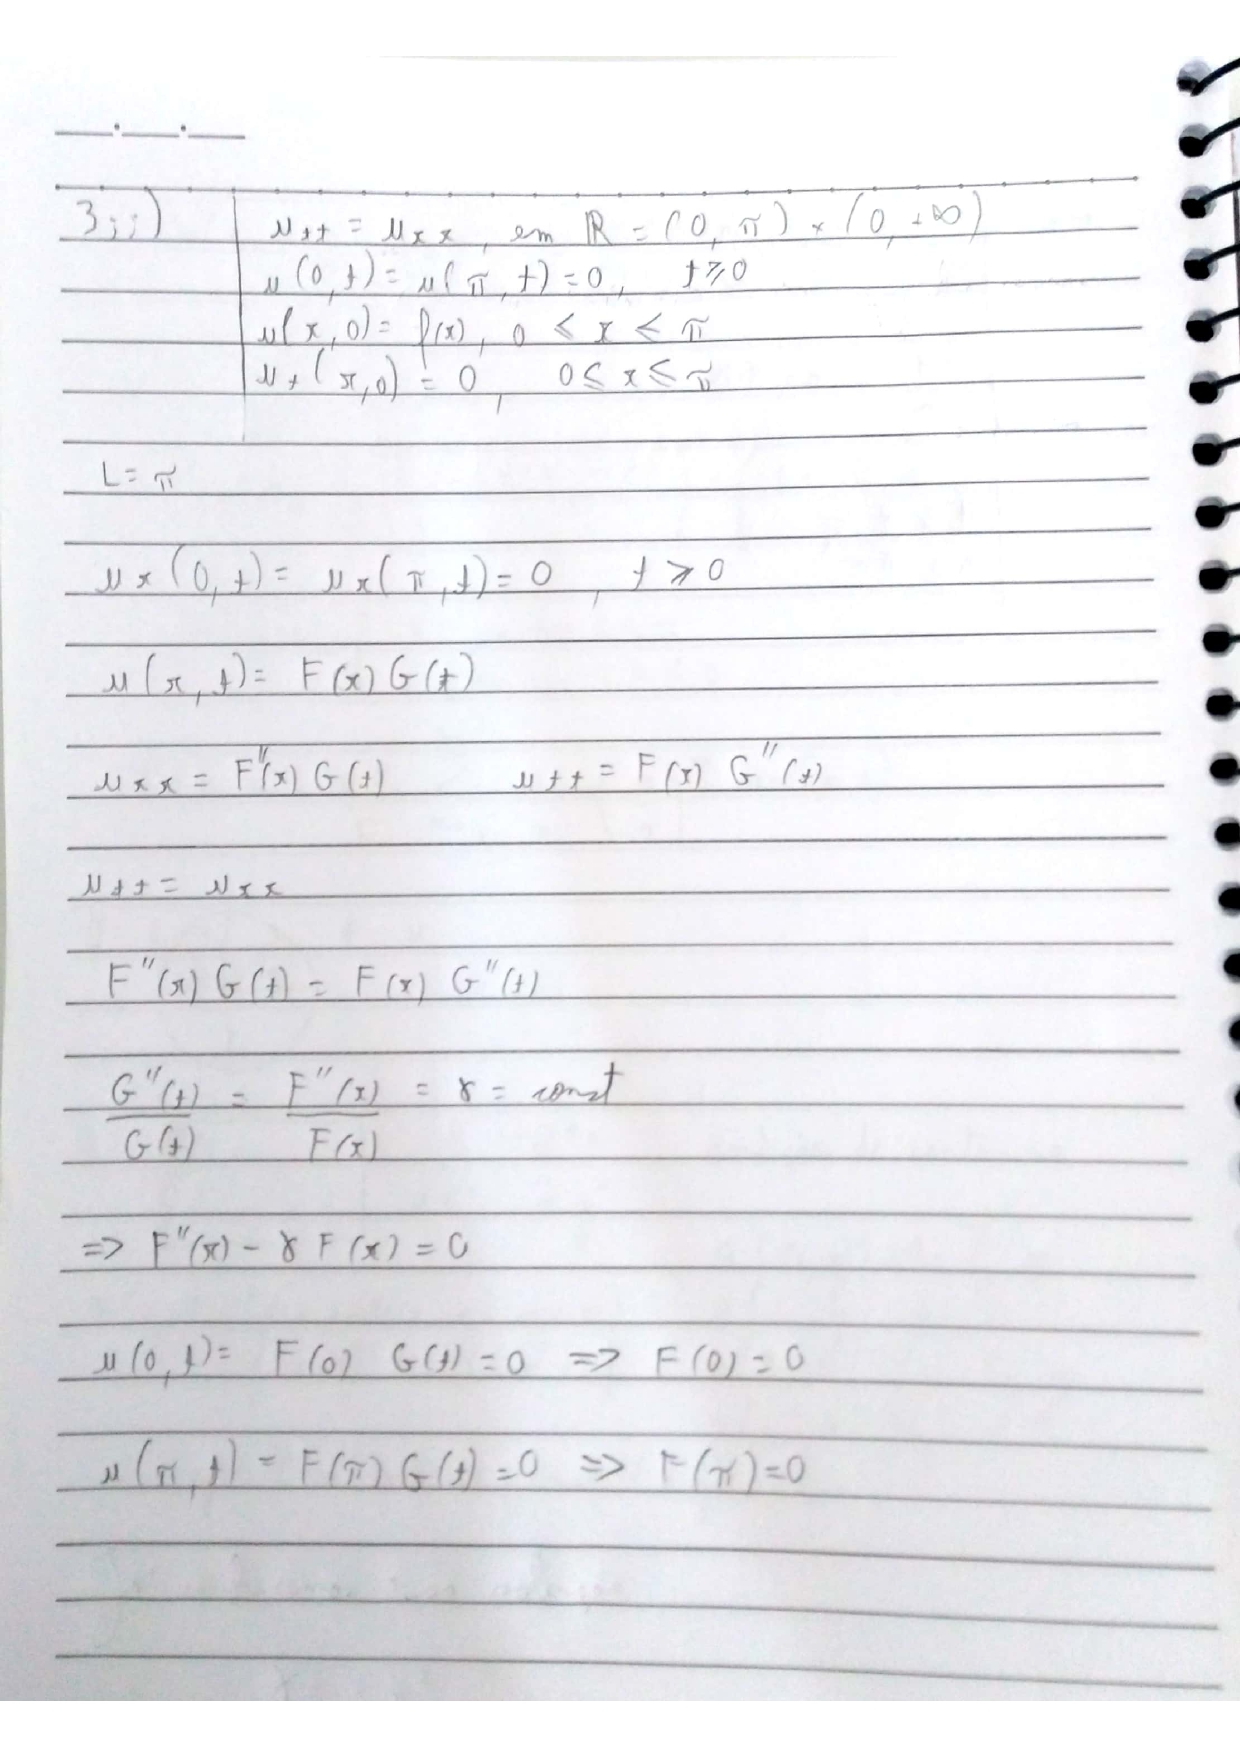
\includegraphics[width=\textwidth]{Questoes-1-3_page-0013.jpg}
        \end{wrapfigure}
        \begin{wrapfigure}{\textwidth}
            \centering
            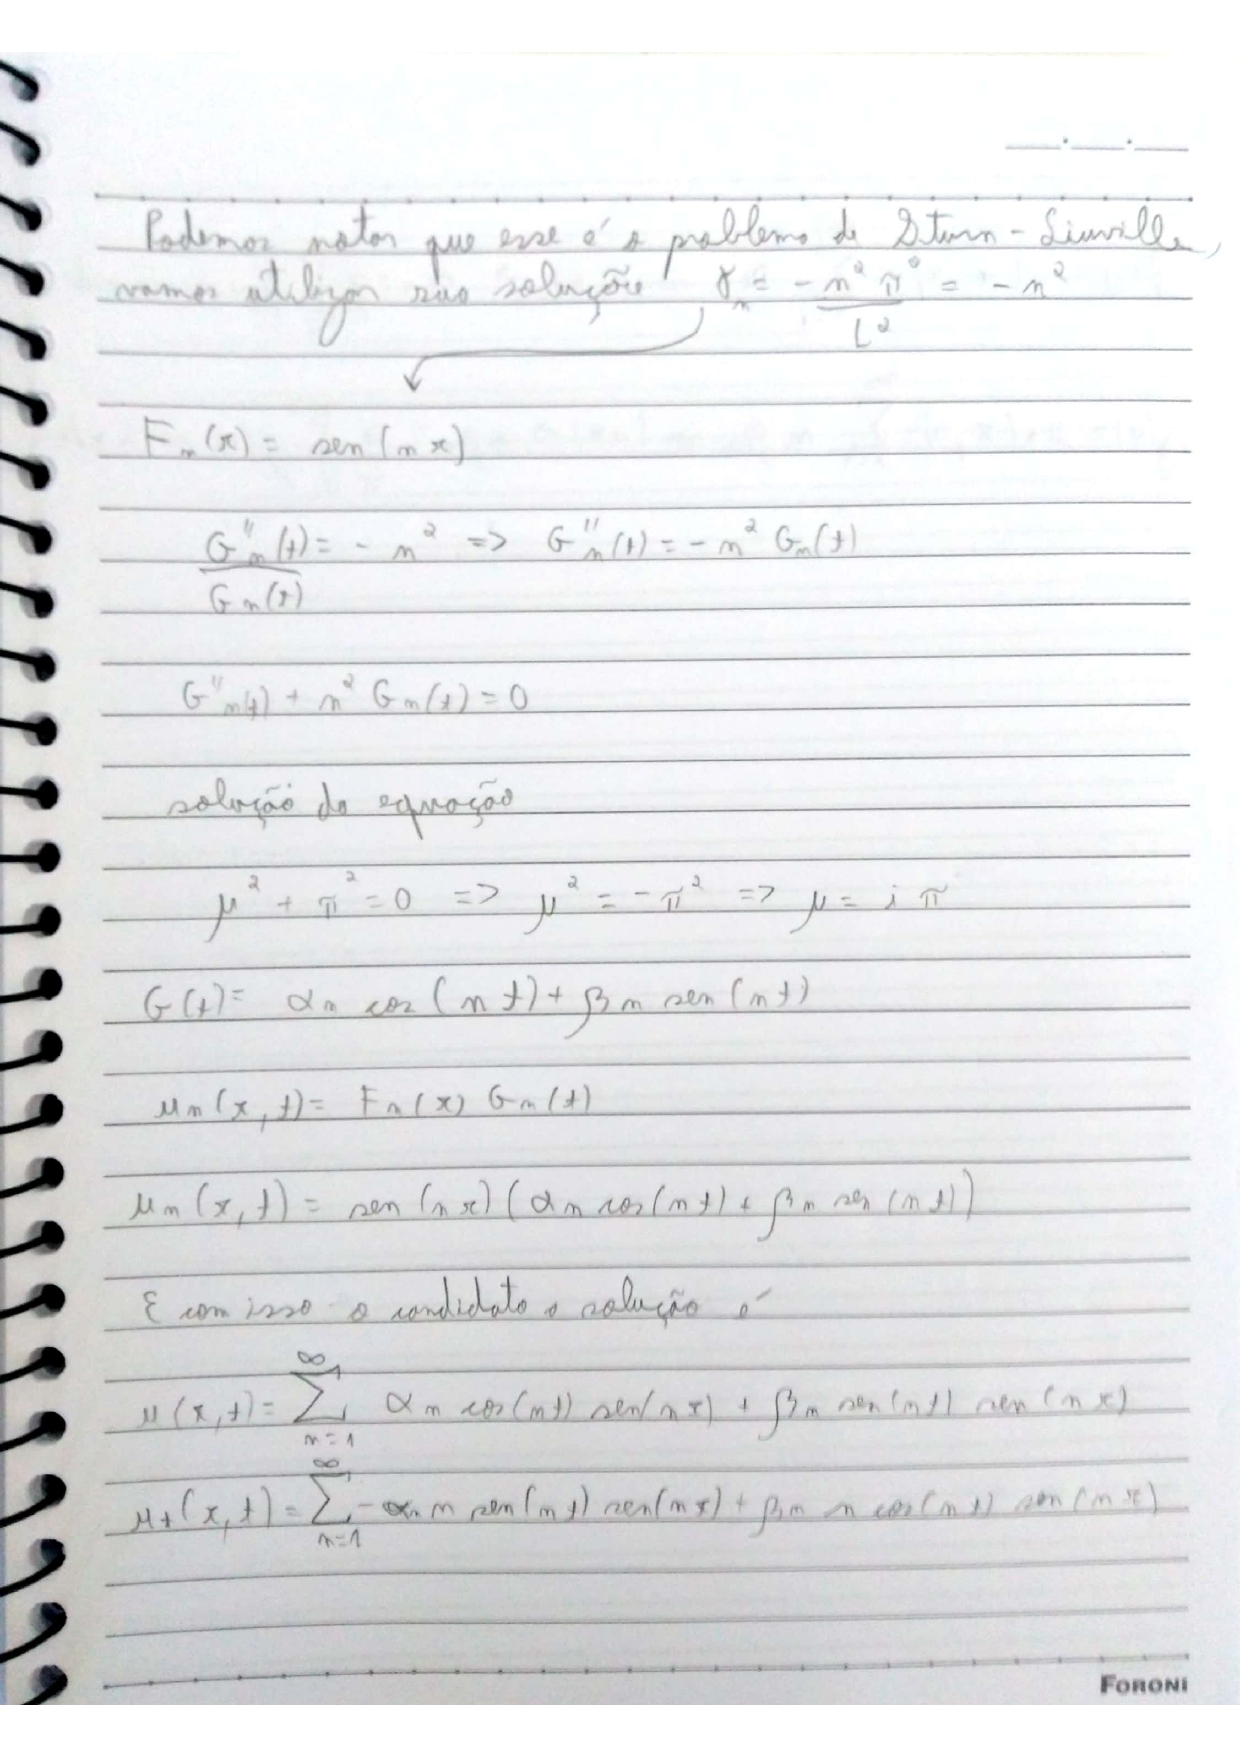
\includegraphics[width=\textwidth]{Questoes-1-3_page-0014.jpg}
        \end{wrapfigure}
        

    \section{ }
        \begin{wrapfigure}{\textwidth}
        \centering
        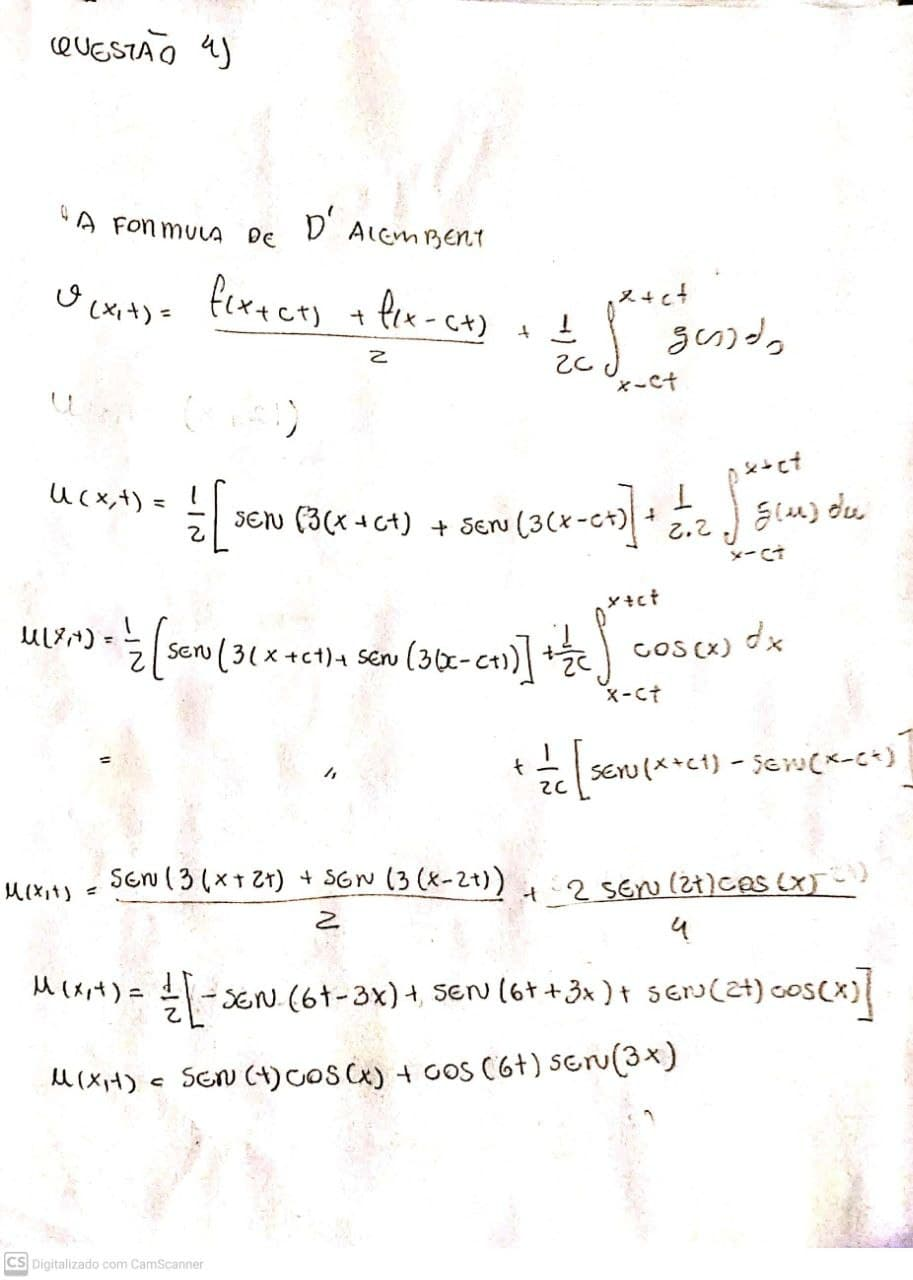
\includegraphics[width=\textwidth]{4.jpg}
    \end{wrapfigure}

\end{document}
